% \chapter{Наука и Техника}


\section{Компьютер}
\textbf{Компьютер и его история.} Компьютеры появились в жизни людей не так давн\'{о}. В середине 20 века простые люди не имели понятия о них. В 1951 году был внедрён первый \explain{коммерчески доступный}{commercially available} компьютер. В 1975 году появились персональные компьютеры.

\textbf{Важность компьютеров.} Трудно представить современную жизнь без компьютеров. Сфера их \explainDetail{применения}{применение}{application} очень широк\'{а}.
Большинство офисов оснащен\'{о} компьютерами для вычислений и работы с документацией. Ранее недоступные хирургические операции сегодня выполняются благодаря компьютерным технологиям. Технологии также внедрены в современном образовании, ими пользуются как студенты, так и преподаватели.

\textbf{Роль компьютеров в жизни подростков.}
Они используют компьютеры для различных целей. Во-первых, играют в компьютерные игры, смотрят мультфильмы и фильмы. Во-вторых, делают школьные задания, читают книги и находят различную информацию в интернете.

\explainDetail{Сравн\'{и}тельно}{сравн\'{и}тельно}{relatively} новая тенденция --- общение онлайн. Такие \explainDetail{приложения}{приложение}{computer application}, как Skype, позволяют в режиме реального времени общаться с людьми, которые находятся очень далеко.

\textbf{Угрозы, связанные с компьютерами.}
Компьютеры оказывают не только положительное влияние на детей. Одна из \explainDetail{угроз}{угр\'{о}за}{threat} --- \explain{вовлечение}{involvement} в виртуальную реальность. Некоторые дети так много времени пров\'{о}дят за компьютером, что забывают о реальных л\'{ю}дях вокруг них.

В результате они будут лишены важных социальных \explainDetail{н\'{а}выков}{н\'{а}вык}{skill} в будущем. Сидя за компьютером, дети портят глаза и осанку. Поэтому взрослые должны быть очень внимательны к тому, как долго их дети пользуются компьютерами.



\clearpage
\section{Северное сияние}
С \explainDetail{наступлением}{наступление}{adventб beginning} осени тысячи туристов \explain{устремляются}{rush} в \explain{Заполярье}{the region of the Arctic circle}, чтобы увидеть уникальный танец небесных огней -- полярное, или северное сияние, на латыни -- Aurora Borealis.
В теории увидеть это природное явление можно с конца августа до середины апреля: в этот период времени ночи становятся темными, солнечная активность \explainDetail{возрастает}{возрастать/возрасти}{возраст\'{а}ю/-ешь/-ет; возраст\'{у}/-ёшь/-\'{у}т: rise, increase}, а облака \explainDetail{расс\'{е}иваются}{рассеиваться/рассеяться}{to disperse}.
Такое развлечение, как \explain{ох\'{о}та}{hunting} за северным сиянием, с каждым годом становится все популярнее как среди россиян, так и среди иностранных туристов, которые специально ради него готовы ехать на Крайний Север. Главное \explain{доказательство}{proof} удачной охоты -- это, конечно же, снимки северного сияния.

\clearpage
\section{Только дьявол мог выдумать Нобелевскую премию}
% https://www.gazeta.ru/science/2015/11/27_a_7914947.shtml
Екатерина Шутова

\textit{120 лет назад Альфред Нобель подписал \explain{завещ\'{а}ние}{will} по Нобелевской премии.}

120 лет назад Альфред Нобель подписал завещание, согласно которому его \explain{накопл\'{е}ния}{accumulation} поступили в фонд Нобелевской премии -- самой престижной на сегодняшний день \explainDetail{награды}{нагр\'{а}да}{prize}, ежегодно \explainDetail{присуждаемой}{присужд\'{а}емый}{awarded} за выдающиеся научные исследования, революционные изобретения или крупный \explain{вклад}{contribution} в культуру или развитие общества. \explainDetail{Отдел}{отдел}{department} науки «Газеты.Ru» вспоминает \explainDetail{подробности}{подробность}{detail} этого события.

В 1888 году журналисты \explain{оповестили}{notified} мир о смерти Альфреда Нобеля -- химика, инженера и изобретателя динамита. Репортеры ошиблись -- на самом деле погиб Людвиг Нобель, брат Альфреда.

\begin{fancyquotes}
    Удивленный изобретатель прочитал в одной из газет собственный некролог под названием «Торговец смертью мертв».
\end{fancyquotes}

Альфред Нобель не захотел оставаться злодеем в глазах человечества. Поэтому 27 ноября 1895 года в Шведско-Норвежском клубе в Париже ученый составил следующее завещание:

{\it
Я, \explain{нижеподписавшийся}{undersigned}, Альфред Бернхард Нобель, обдумав и решив, настоящим объявляю мое завещание по поводу имущества, нажитого мною... Капитал мои душеприказчики должны перевести в ценные бумаги, создав фонд, проценты с которого будут выдаваться в виде премии тем, кто в течение предшествующего года принес наибольшую пользу человечеству.

Указанные проценты следует разделить на пять равных частей, которые предназначаются: первая часть тому, кто сделал наиболее важное открытие или изобретение в области физики, вторая --- в области химии, третья --- в области физиологии или медицины, четвертая --- создавшему наиболее значительное литературное произведение, отражающее человеческие идеалы, пятая --- тому, кто внесет весомый вклад в сплочение народов, уничтожение рабства, снижение численности существующих армий и содействие мирной договоренности.

... Мое особое желание заключается в том, чтобы на \explain{присуждение}{awarding, conferment} премий не \explainDetail{влияла}{влиять/повлиять}{influence} национальность кандидата, чтобы премию получали наиболее \explain{достойные}{worthy}, независимо от того, скандинавы они или нет.}

\subsection{Как огорчить родственников}
Спустя год после написания завещания Альфред Нобель скончался на своей вилле от \explainDetail{кровоизлияния}{кровоизлияние}{hemorrhage} в мозг. За несколько лет до смерти ученый сказал о самом себе следующим образом: «Альфред Нобель -- его \explain{существование}{existence} следовало бы \explain{пресечь}{suppress} при рождении милосердным доктором. Основные добродетели: держит ногти в чистоте и никому не бывает в тягость. Основные недостатки: не имеет семьи, наделен дурным характером и плохим пищеварением.

\begin{fancyquotes}
    Величайший грех: не поклоняется Мамоне. Важнейшие события в его жизни: никаких.
\end{fancyquotes}

\explain{Наследники}{heirs} легендарного изобретателя были крайне \explain{возмущены}{outraged}, что огромные накопления уйдут не им в карман, а на поддержку науки. Они требовали, чтобы завещание было признано недействительным. Интересно, что единственным родственником Нобеля, не пытавшимся присвоить себе деньги, оказался его племянник Эммануил. «Русские называют исполнителя завещания «душеприказчик», то есть «представитель души», --- заявил юристам мужчина. --- Вот и действуйте соответственно». Позднее Эммануил добавил: «Я не хочу, чтобы достойнейшие ученые в будущем упрекали нашу семью в присвоении средств, которые по праву принадлежат им».

В конечном итоге справедливость восторжествовала --- и через несколько лет после смерти ученого были вручены пять первых премий. А с 1969 года по инициативе Шведского банка начала присуждаться Нобелевская премия по экономике.

Лишь однажды деньги из фонда премии пошли на дело, никак не связанное с наукой. Софи фон Капивара, женщина, с которой у талантливого изобретателя были отношения, пообещала раскрыть содержание их переписки и посмертно опозорить Альфреда Нобеля. Душеприказчики в страхе выплатили крупную сумму за 216 писем мецената. Ученые до сих пор шутят, что

\begin{fancyquotes}
    наука была бы богаче, если бы не одна алчная молочница.
\end{fancyquotes}

«Ты славная девушка, но ты действуешь мне на нервы»

Существует миф, согласно которому у Альфреда Нобеля была жена, страстно влюбившаяся в математика, и именно поэтому изобретатель «обделил» всех представителей этой науки. Но на самом деле, как заявляют биографы, меценат никогда не был женат. В молодом возрасте Нобель влюбился в работницу аптеки, но та умерла от чахотки. Потосковав, ученый нашел новую пассию --- на этот раз ей стала Сара Бернар, знаменитая актриса. Альфред Нобель написал письмо матери о том, что хочет жениться.

\begin{fancyquotes}
    Недаром актеров в старину не разрешали хоронить на кладбище. У них нет души, сыночек!» --- предупредила сына любящая родительница.
\end{fancyquotes}



Послушный Нобель разорвал любовную связь с Бернар.

Следующая женщина появилась в жизни мецената, когда тому уже был 41 год. Альфред Нобель опубликовал в газете объявление о том, что ищет секретаршу. На него откликнулась графиня Берта Кински, с которой у изобретателя начался неторопливый и гармоничный роман.

\begin{fancyquotes}
    Кстати, по одной из версий, именно Кински попросила Нобеля вписать в завещание премию мира. А в 1905 году она стала первой женщиной, удостоенной этой премии.
\end{fancyquotes}

У Кински и Нобеля дело до свадьбы не дошло: однажды ученый обнаружил, что его секретарша исчезла, оставив на столе письмо следующего содержания: «Простите меня, господин Нобель. Я уезжаю в Вену, где меня ждет жених. Пожелайте мне счастья, как я желаю счастья вам. Искренне преданная вам Берта Кински, которая в скором времени станет Бертой фон Зуттер».

Последней женщиной в жизни Нобеля стала вышеупомянутая «алчная молочница», которая изрядно надоедала ученому своей глупостью и необразованностью. «Дорогое дитя. Ты славная девушка, но ты действуешь мне на нервы», --- раздраженно писал ей в письмах Альфред Нобель.

Так почему же не существует премии по математике? Возможно, все дело в том, что у Альфреда Нобеля не заладились отношения с великим математиком Миттаг-Леффлером, который должен был стать первым лауреатом, а меценат этого не хотел. Но наиболее вероятная версия заключается в том, что Нобель воспринимал математику как инструмент, как сугубо теоретическую науку.

\subsection{Виагра для хомячков и исследование ругани}

В 1991 году появилась пародия на Нобелевскую премию --- Шнобелевская премия. Она вручается «за достижения, которые заставляют сначала засмеяться, а потом --- задуматься». Учредитель и идейный вдохновитель «Шнобелевки» --- Марк Абрахамс, который, будучи редактором юмористического научного журнала, получал множество писем от читателей с подробным рассказом об их «великих» исследованиях. «Иногда эти люди заслуживали премии --- правда, не Нобелевской», --- говорил Абрахамс. Так редактор решил награждать ученых за самые нелепые достижения.

В разные годы Шнобелевская премия присуждалась

за разработку протезов яичек для собак, за исследование влияния музыки кантри на частоту самоубийств и за открытие, что «Виагра» помогает хомякам справиться с последствиями резкой смены часовых поясов.

Также пародийную награду получали ученые, доказавшие, что ругань снижает боль, и исследователи, изучавшие оральный секс у летучих мышей.

Первым в мире человеком, удостоенным как Шнобелевской, так и Нобелевской премии, стал Андрей Гейм. Голландский ученый российского происхождения был награжден «Шнобелевкой» за использование магнитов для того, чтобы демонстрировать возможность левитации лягушек. Спустя десять лет Гейм совместно со своим учеником Константином Новоселовым получил Нобелевскую премию за изобретение графена.

\subsection{Война еще не закончена, а премии уже раздают}
«Я готов простить Альфреду Нобелю изобретение динамита, но только дьявол в людском обличье мог выдумать Нобелевскую премию!» --- воскликнул ирландский романист и драматург Джордж Бернард Шоу, став лауреатом в области литературы (по ироничному заявлению писателя, произошло это потому, что «в тот год он ничего не опубликовал»). Действительно, самая престижная международная награда --- явление весьма резонансное и неоднозначное. В Советском Союзе Нобелевский комитет клеймили за то, что «он ухитрился не заметить Алексея Толстого, Максима Горького, Владимира Маяковского, но зато заметил Ивана Бунина. И только тогда, когда он стал эмигрантом, и только потому, что он стал эмигрантом и врагом советского народа».

В Третьем рейхе ученым было запрещено получать Нобелевскую премию, так как в 1935 году премию мира «За борьбу с милитаризмом в Германии» получил пацифист Карл фон Осецкий --- ярый противник нацистского режима. В 1937 году Адольф Гитлер издал указ, согласно которому немцы не имели права принимать премию. Из-за указа награду не получили Герхард Домагк «за открытие антибактериального эффекта пронтозила», Адольф Бутенандт за исследование половых гормонов и Рихард Кун за работу по каротиноидам и витаминам.


\begin{fancyquotes}
    Весьма примечателен тот факт, что Бенито Муссолини и Адольф Гитлер были номинированы на Нобелевскую премию мира в 1935 и 1939 годах соответственно.
\end{fancyquotes}

Нобелевская история знает немало случаев отказа от самой престижной международной награды.

Так, в 1973 году политический деятель Фан Динь Кхай отказался от медали «за работу по разрешению вьетнамского конфликта», аргументируя свое решение тем, что «война еще не закончена, а премии уже раздают». Не захотел быть награжденным и Жан-Поль Сартр --- французский писатель и драматург. По мнению Сартра, награда посягнет на его независимость --- центральное понятие в философии автора. Вскоре после отказа от Нобелевской премии француз еще раз шокировал общественность, заявив, что уходит из литературы. «Литература --- суррогат действенного преобразования мира», --- с горечью заметил писатель.

\clearpage
\section{Ученые нашли способ записать данные в пяти измерениях}

\textit{Как 5D-диски изменят представление людей о хранении информации?}

\textbf{Ученые создали 5D-диск высочайшей плотности:} В октябре специалисты Саутгемптонского университета в Великобритании описали способ записи огромного количества данных на компактный диск небольших размеров. Технология, получившая название 5D, позволяет сохранить на специальном накопителе до 500 терабайт информации. Получившиеся диски из кварцевого стекла отличаются высочайшей плотностью, которая в десять тысяч раз превышает плотность оптических дисков Blu-Ray. Новый метод позволит эффективно разместить на небольшой площади облачные сервера для хранения данных пользователей, интернет-компаний, крупных корпораций. По словам ученых, это особенно важно на фоне развития технологий, увеличения количества подключенных к сети устройств и роста количества передаваемых через сеть данных.

\textbf{Облачные сервисы с каждым годом становятся все популярнее:}
За последние пять лет отношение потребителей и бизнеса к облачным сервисам изменилось. Раньше их воспринимали в качестве дополнительного метода резервного копирования данных --- информация практически всегда поступала в одну сторону. Причем крупные корпорации в основном использовали дата-центры для хранения некритичной информации. К 2020-м годам организации стали использовать облачные серверы не только для аварийного копирования, но и для постоянного обмена данными внутри конкретного предприятия. Системы облачных хранилищ стали более гибкими, позволяя конкретному потребителю выбрать необходимое количество свободного места и производительность оборудования.

Специалисты Analytics Insight называют основными \explainDetail{преим\'{у}ществами}{преим\'{у}щество}{advantage} \explainDetail{облачных}{облачный}{cloud (adj.); \'{о}блако: cloud} дата-центров \explain{круглос\'{у}точный}{round the clock} доступ к информации, возможность одновременной работы не- скольких пользователей с одним массивом данных, масштабируемость и \explain{г\'{и}бкость}{flexibility}, \explain{снижение}{decline} затрат на хранение данных внутри компании.

\explainDetail{Представители}{представитель}{representative} отрасли отмечают, что в обычное время нагрузка на серверы неравномерна: в одной части дата-центров она может зашкаливать, в другой быть крайне небольшой. По этой причине эксперты предсказывают появление искусственного интеллекта, который мог бы анализировать и распределять нагрузку на оборудование. В том числе по этой причине данные пользователей хранятся в нескольких частях дата-центра.

\textbf{Больше всего в облачных сервисах пользователи ценят скорость передачи данных и безопасность:} По словам основателя облачного провайдера Wasabi Дэйва Френда, от дата-центров будущего потребители ожидают высокого уровня безопасности, производительности оборудования и приемлемой цены за услуги. «Резервные копии должны храниться в разрозненных системах, обеспечивающих максимально возможную изоляцию», --- заметил предприниматель. Потенциальный злоумышленник, добравшийся до одного сервера, не должен иметь возможность удалить или зашифровать информацию так, чтобы ее нельзя было восстановить из альтернативных источников. Френд полагает, что на этом должна строиться концепция мультиоблака.

Другими критериями облачного сервиса будущего, по мнению Френда, являются доступная цена и высокая скорость передачи данных. Провайдеры должны будут таким образом скорректировать стоимость услуг и добиться определенного качества оборудования, чтобы оставаться конкурентоспособными и не разочаровывать клиентов.

Представители облачного провайдера CloudSigma рассказали, что дата-центры должны будут отвечать за сохранность данных и скорость передачи информации. Для хранения файлов пользователей и корпоративных клиентов они используют небольшие 2,5-дюймовые диски емкостью 250 гигабайт. В случае, если какой-либо диск выходит из строя, его заменяют, а данные восстанавливают через бэкап. При таком развитии событий клиент не теряет своих данных, хотя и оказывается без доступа к информации на 10-15 минут. Благодаря глубокой интеграции между серверами и оборудованием задержка передачи данных внутри дата-центра очень мала. Для того чтобы разогнать скорость и снизить задержку между серверами и пользователем, в компании полагаются на выделенную гигабитную линию интернета.


\textbf{Диски 5D позволят хранить информацию практически бесконечно:}
По оценке Forbes, к 2025 году к интернету будет подключено около 80 миллиардов устройств, которые будут генерировать около 180 триллионов гигабайт данных. В обозримом будущем хранить данные на классических накопителях будет проблематично --- существует риск возникновения дефицита и увеличения стоимости хранения информации. Работающие над технологией 5D специалисты Саутгемптонского университета предлагают записывать информацию на кварцевом стекле с помощью фемтосекундных лазеров и сверхкоротких импульсов. «Запись на кварцевый носитель как бы идет в пяти измерениях --- двух оптических и трех пространственных», --- отмечают авторы исследования.

Инновация британских инженеров заключается в создании дисков повышенной плотности и размещении на небольшом участке колоссальных объемов данных. Например, на «болванке» размером в один дюйм удалось сохранить шесть гигабайт информации. Накопитель обычного для подобных устройств размера, основанный на кварцевых дисках, может сохранить до 500 терабайт данных. Разработка обещает революцию на рынке хранения информации, так как десятки, если не сотни классических дата-центров можно будет объединить в одну библиотеку.

Преимуществами 5D-дисков также называют долговечность и низкую стоимость обслуживания. По оценке ученых, кварцевые диски не прочнее обычных накопителей, однако могут выдержать температуру до 1800 градусов по Фаренгейту, или около тысячи градусов по Цельсию. В случае пожара в дата-центре информация, скорее всего, сохранится. Кроме того, кварцевое стекло со временем не меняет своих свойств, что позволит держать данные на 5D-накопителях практически вечно.

Единственным узким местом будущей разработки является скорость передачи данных. В настоящий момент ученым удалось разогнать ее до 230 килобайт в секунду --- за это время на диск можно записать около ста страниц текста. Однако для того, чтобы полностью заполнить болванку емкостью 500 терабайт, потребуется 60 дней. Либо инженеры найдут способ обойти ограничение, либо 5D-диски так и останутся перспективным оборудованием для записи информации. В крайнем случае на подобных дисках можно сохранять данные для потомков. Так, в 2018 году на кварцевый носитель была записана трилогия романов Айзека Азимова «Основание» --- диск отправился в космос вместе с Tesla Roadster Илона Маска.


\clearpage
\section{У коронавируса есть механизм самоуничтожения}
% https://russian.rt.com/science/article/937351-pyotr-chumakov-intervyu-virusy
\textit{Пётр Чумаков об эволюции SARS-CoV-2 и лечении вирусами}

\explainDetail{Снижение}{снижение}{decrease} патогенности новых \explainDetail{штаммов}{штамм}{strain (of virus)} SARS-CoV-2 \explain{предопределено}{predetermined} самой логикой эволюции вирусов такого типа. Об этом в интервью RT рассказал член-корреспондент \explain{РАН}{Российская академия наук}, профессор и главный научный сотрудник Института молекулярной биологии РАН Пётр Чумаков. Он также отметил, что многие вирусы можно поставить на службу человеку: например, использовать их непатогенные варианты для защиты людей от опасных \explainDetail{возбудителей}{возбудитель}{pathogen}. За вакцинами, основанными на этом принципе, будущее, считает учёный. По его мнению, вирусы можно использовать и для лечения рака.

{\bf --- С самог\'{о} \explain{начала}{from начало (\textit{суш.}): start, beginning} пандемии многие боялись появления \explain{ос\'{о}бо}{especially, particularly} \explainDetail{смертоносного}{смертоносный}{deadly} штамма вируса. Почему этого пока не случилось? По \explainDetail{предварительной}{предварительный}{preliminary} информации, новый штамм «омикрон» не привёл к \explainDetail{резкому}{резкий}{sharp} росту \explainDetail{летальности}{летальность}{lethality}. Да и в целом опасные мутации \explainDetail{распространённых}{распространённый}{widespread} вирусов случаются не очень часто --- например, даже грипп вызвал смертельную пандемию только один раз, в начале XX века.}

--- Коронавирус SARS-CoV-2 --- новая для человека инфекция. Она перешла в человеческую популяцию только два года назад. До этого коронавирус этого типа циркулировал в основном среди \explainDetail{летучих мышей}{летучая мышь}{bat}. Эти животные \explainDetail{обладают}{обладать}{possess} очень сильной противовирусной защитой, организм летучих мышей заточен для противостояния инфекциям, поскольку они живут в очень \explainDetail{скученных}{скученный}{crowded} колониях. Вирусы, которые способны \explain{пробить}{pierce} эту защиту, должны также быть \explain{вооружены}{armed} очень серьёзными системами преодоления противовирусного иммунитета. И когда такой вирус попадает к человеку, он вызывает тяжёлые \explainDetail{заболевания}{заболевание}{disease}, потому что человеческая иммунная противовирусная система слабее, чем у летучих мышей.

Однако, попав в организм человека, такой вирус тоже должен \explain{приспособиться}{adapt} к новым условиям. Поэтому первые фазы эволюции вируса --- это \explain{накопление}{accumulation} таких мутаций, которые будут приводить к его более эффективному \explainDetail{размножению}{размножение}{reproduction} в организме человека. Это \explain{сопровождается}{is accompanied by} ростом инфекционности и усилением патогенных \explainDetail{свойств}{свойство}{property}. Когда вирус активно размножается, он приспосабливается к организму человека и действует более эффективно.

Вторая фаза эволюции вируса --- аттенуирование. Это приспособление вируса к организму при \explainDetail{ослаблении}{ослабление}{weakening} его патогенности.

При этом инфекционность может расти, потому что вирусу важно быстро \explainDetail{распространяться}{распространяться/распространиться}{spread} на новом хозяине. Однако \explain{излишняя}{superfluous, excessive} патогенность ему не нужна. Дело не в том, что вирус \explain{якобы}{ostensibly} знает, что ему невыгодно убивать человека. Нет, просто это качество --- патогенность --- не востребовано в организме человека и поэтому постепенно ослабевает при накоплении мутаций. В результате вирус вызывает всё меньше летальных исходов и тяжёлых случаев.

\begin{fancyquotes}
    Сейчас штамм коронавируса «омикрон» является примером второй фазы эволюции вируса, \explain{наблюдается}{is observed} его аттенуирование при одновременном увеличении \explain{заразности}{infectiousness}. Итогом должно стать превращение коронавируса в обычное сезонное вирусное заболевание.
\end{fancyquotes}

В случае с «омикроном» примечательна внезапность его появления, он сразу накопил 32 мутации по сравнению с предыдущим штаммом. В Африке очень много иммунодефицитных людей, и, по всей видимости, новый штамм \explainDetail{возник}{возникать/возникнуть}{arise (возн\'{и}к, возн\'{и}кла, возн\'{и}кло, возн\'{и}кли)} в организме именно такого человека. В его организме он прошёл тот путь эволюции, который обычно вирус проходит через большую \explainDetail{цепочку}{цепочка}{chain} \explainDetail{заражений}{заражение}{infection}. В итоге в ускоренном режиме этот вирус превратился в менее патогенный вариант.

Впр\'{о}чем, я бы не хотел никого \explainDetail{расхолаживать}{расхолаживать/расхолодить}{discourage}, говоря о том, что бояться нечего. Нет. Пока что это --- лишь оптимистичный сценарий. Мы пока не имеем достаточного числа случаев заболевания этим штаммом, чтобы заявлять о его низкой опасности. Да, по предварительным данным, пока что от него никто не умер. Но нужно понаблюдать за тем, как будет развиваться ситуация, и продолжать вакцинироваться. Потому что даже если оптимистичный сценарий верный, нельзя исключать, что штамм «омикрон» неожиданно исчезнет, как исчез в Японии штамм «дельта».

\explainDetail{По видимости}{по видимости}{apparently}, у коронавируса есть механизм самоуничтожения. Это может случиться и со штаммом «омикрон», а ему на смену придут более \explain{болезнетворные}{pathogenic} варианты.

{\bf --- Как вакцинация \explainDetail{влияет}{влиять/повлиять}{influence} на мутации вируса --- насколько она снижает их вероятность, \explain{учитывая}{considering, taking into account}, что вакцинированные тоже болеют, пусть и в лёгкой форме?}

--- \explainDetail{Особенность}{особенность}{peculiarity} этого коронавируса в том, что даже очень иммунные люди, которые перенесли заболевание или вакцинированы, могут заразиться \explain{повт\'{о}рно}{repeatedly}, даже не чувствуя при этом симптомов. При этом вирус будет выделяться из носоглотки. Однако вероятность мутаций вируса в такой ситуации всё же не очень велика. Гораздо чаще новые варианты вируса возникают в организмах больных людей, особенно иммунодефицитных.

{\bf --- Вы \explainDetail{упомян\'{у}ли}{упомин\'{а}ть/упомян\'{у}ть}{to mention, to refer} феномен \explainDetail{исчезновения}{исчезнов\'{е}ние}{disappearance} «дельты» в Японии. Не могли бы рассказать об этом \explain{подробней}{in more detail (detail: подробность)}? Случалось ли подобное когда-то раньше?}

--- Нет, это новая гипотеза одного из японских исследователей. Гипотеза, на первый взгляд, экстравагантная. Потому что обычно эволюция идёт таким путём, что \explain{выживает}{survives} сильнейший --- наиболее \explain{жизнеспособный}{viable}. А в этом случае произошло, напротив, эволюционное самозатухание вируса. Согласно гипотезе, это связано с мутацией в гене NSP-14. Это один из неструктурных \explainDetail{белков}{бел\'{о}к}{protein} коронавируса, не входящий в состав вирусной \explainDetail{част\'{и}цы}{част\'{и}ца}{particle}. Он нужен для поддержания репликации вируса, корректирует правильность считывания генома, исправляет ошибки. Если этот белок не функционирует, то вирус начинает с большой \explainDetail{скоростью}{скорость}{speed} накапливать мутации, включая летальные. Они приводят к тому, что вирус уже не может размножаться.

Не знаю, \explain{подтвердится}{confirmed} ли эта гипотеза, однако, когда в Японии секвенировали варианты коронавируса до того, как он исчез, оказалось, что там действительно были мутации белка NSP-14.

Более того, предыдущая \explain{вспышка}{outbreak} SARS-1 в 2003 году тоже \explain{затухла}{faded} сама по себе, её даже не успели подавить вакциной.

Что касается «омикрона», я пока не видел никаких данных о том, что у него \explain{повреждён}{damaged} белок NSP-14. Однако этого нельзя исключать, это объяснило бы скорость накопления в нём мутаций.

{\bf --- Ещё говорят, что штамм «омикрон» очень сильно отличается от других штаммов и что в нём нашли элемент генома человека, который также есть в вирусе \explainDetail{простуды}{простуда}{common cold}. И что это делает его менее заметным для иммунной системы.}

--- Нет, что это элемент генома человека --- это ерунд\'{а}. Это маленькая вставка. И когда мы говорим о \explainDetail{посл\'{е}довательности}{посл\'{е}довательность}{sequence}, \explain{допуст\'{и}м}{let's say}, трёх \explainDetail{аминокислот}{аминокислот\'{а}}{aminoacid}, такая посл\'{е}довательность может встречаться и в человеке, и в растении --- \explain{где угодно}{anywhere}.

{\bf --- Нед\'{а}вно вы сказали, что омикрон-штамм может выступить в качестве естественной вакцины. А были такие прецеденты раньше?}

---  Может быть, были, но они не зафиксированы. Однако что такое «живая вакцина»? Это просто вирус, который не имеет высокой патогенности, но \explain{вызыв\'{а}ет}{causes} иммунный ответ. Обычно такой непатогенный штамм делают искусственно. Например, полиомиелитная вакцина была создана путём селекции, были отобраны вирусы, которые \explainDetail{утратили}{утрачивать/утратить}{to lose} способность \explainDetail{поражать}{пораж\'{а}ть/пораз\'{и}ть}{to hit, to affect} нервные \explainDetail{кл\'{е}тки}{кл\'{е}тка}{cell}. При этом они хорошо размножаются в \explainDetail{кишечнике}{кишечник}{intestine} и вызывают \explain{стойкий}{persistent} иммунитет против полиомиелита. Живая вакцина против \explainDetail{кори}{корь}{measles} тоже была создана на основе патогенного вируса кори, который приобрёл свойства непатогенности.

Природа тоже может создавать такие вирусы. И природная аттенуация вирусного штамма --- это, \explain{по с\'{у}ти}{in fact}, именно такой процесс. Такой вирус \explain{вытесняет}{displaces} патогенные варианты и создаёт иммунную прослойку, которая уже не \explainDetail{позволяет}{позвол\'{я}ть/позв\'{о}лить}{to allow, to permit (also: разреш\'{а}ть/разреш\'{и}ть)} новому патогенному варианту вызвать заболевание.

{\bf --- Ранее в Университете Глазго провели исследование, в результате которого \explain{в\'{ы}яснилось}{it turned out}, что люди очень редко болеют одновременно двумя вирусными заболеваниями. Однако точное объяснение этого тогда найти не удалось. Есть ли сейчас какие-то гипотезы на этот счёт? И можно ли использовать «конкуренцию» вирусов в полезных целях, существуют ли подобные проекты?}

--- Да, есть такое правило, хотя из него тоже бывают исключения. В основе этого явления лежит феномен интерференции. Когда человек или животное \explain{заражается}{gets infected (+\textit{твор.})} вирусом, в ответ в организме \explain{выраб\'{а}тывается}{produced} интерферон --- противовирусный бел\'{о}к. Он циркулирует по всем\'{у} организму, клетки в ответ вырабатывают противовирусное состояние. И другому вирусу будет уже очень трудно внедриться в организм в это время. Однако некоторые вирусы вырабатывают противодействие интерфероновому механизму --- тогда возможна сочетанная инфекция. Возможно также одновременное заражение двумя вирусами, когда первый вирус ещё не вызвал противовирусное состояние.

{\bf --- А учёные думали над тем, чтобы как-то использовать этот интерфероновый механизм для борьбы с болезнями?}

--- Конечно. Такие исследования проводились в 1970-е годы, я принимал в них участие. Есть целый ряд непатогенных вирусов, которые обычно \explain{обитают}{inhabit} в кишечнике здоровых детей в возрасте от двух до пяти лет. Их испытывали как средство профилактики сезонных простудных вирусных инфекций. В начале 1970-х годов было проведено \explain{масштабное}{large-scale} испытание более чем на 300 тыс. человек в шести городах СССР. В итоге заболеваемость \explain{ОРВИ}{острая респираторная вирусная инфекция: acute respiratory viral infection} среди привитых снизилась в 3,5 раза. Это очень хороший результат, такой же, как у специфических противовирусных противогриппозных вакцин.

\begin{fancyquotes}
    Примечательно, что профилактика, основанная на механизме интерференции, защищает не только от одного вируса, а от многих. Поэтому такая неспецифическая профилактика очень важна именно в случае появления новых инфекций, чтобы выиграть время до создания специфической вакцины.
\end{fancyquotes}

Тем более что такие препараты применяются в виде \explain{капель}{drops}, \explain{перорально}{orally}. Это не будет вызывать такого \explainDetail{отторжения}{отторжение}{rejections} у антиваксеров.

{\bf --- А сейчас разрабатываются новые препараты с этим принципом действия?}

--- У нас есть панель таких вирусов. Но проблема в том, что такие вещи с большим трудом пробивают себе дорогу. Например, нам не удалось \explainDetail{убед\'{и}ть}{убеждать/убедить}{to convince [убеждать: убеждаю, убеждаешь, убеждают]} использовать этот метод во время \explain{нынешней}{current} пандемии. Потому что наш подход очень дешёвый, он не очень интересен для бизнеса. Ведь на выпуск вакцин выделяются большие деньги.

Но я уверен, что мы вступаем в такое время, когда вирусы могут использоваться и в качестве оружия. Поэтому нужно иметь стратегический \explain{зап\'{а}с}{stock, reserve} \explain{экстренных}{emergency} средств защиты. И надеюсь, что в итоге собранный нами запас непатогенных вирусов будет использован и признан в качестве такого средства.

{\bf --- Раз вирусы могут \explain{конкурировать}{compete} и вытеснять друг друга, не рассматривается ли научным сообществом, к примеру, идея создать генно-инженерными методами не опасный, но очень контагиозный штамм SARS-CoV-2, чтобы вытеснить те его штаммы, которые приводят к высокой летальности? }

--- Это отличный вопрос. Вообще я считаю, чтобудущее вакцинологии --- это жив\'{ы}е вакцины. Просто сейчас мы идём \explain{проторённым}{well-trodden} путём, создаём традиционные вакцины. Либо это инактивированный вирус, либо какие-то генные инженерные продукты --- на основе других вирусов.

При этом аттенуированные штаммы можно создать из л\'{ю}бого болезнетворного вируса. Зная, какие гены участвуют в патогенезе, можно внести искусственные изменения и сделать из него такой безопасный вирус, который будет тем не менее иммуногенен и будет защищать от инфекции.

Но, к сожалению, пока что этот путь не всеми признаётся, широких работ в этом направлении не ведётся.

{\bf --- В 2020 году в интервью RT вы рассказали о \explainDetail{разработке}{разработка}{development} модифицированных вирусов, которые вызывают \explain{гибель}{death} раковых клеток. Мы хотели бы вернуться к этой теме. Готовятся ли клинические испытания или они уже проводятся?}

--- Да, эта работа продолжается, у нас есть большая панель онколитических вирусов. Почему нужна целая панель, а не один препарат? Потому что \explainDetail{опухоли}{\'{о}пухоль}{tumour} у людей очень индивидуальны. Допустим, у двух людей рак молочной \explainDetail{железы}{желез\'{а}}{gland} одной и той же гистологической категории. Но на молекулярном уровне это совершенно разные заболевания, там разный набор повреждений. \explain{В том числе}{including} повреждаются такие гены, которые могут быть нужны какому-то конкретному вирусу для его репликации. И он уже не может лечить данную \'{о}пухоль. Но может другой --- его нужно подобрать из панели.

Конечно, такой сложный препарат трудно быстро \explain{внедрить}{to implant, to embed, to introduce}, нужно пройти долгие этапы пров\'{е}рок. К сожалению, регуляторика --- \explain{узкое}{narrow} место для биотерапии. На самом деле правила нужно очень сильно менять, чтобы создание и внедрение таких препаратов происход\'{и}ло быстр\'{е}й.

Пока что \explain{проведены}{$<$ провести} только \explain{доклинические}{pre-clinical} испытания, их итоги подводятся. Возможно, что к концу г\'{о}да будет какое-то заключение. После этого встанет вопрос о том, как организовать клинические испытания. Нужно будет найти инвесторов, собрать пациентов-добровольцев\dots{} Всё это \explain{затягивается}{drags on} на годы.

Тем не менее по своему опыту мы знаем, что эта терапия действует и абсолютно безопасна.

{\bf --- Удалось ли собрать какую-то предварительную статистику?}

--- Собрать корректную статистику пока невозможно, потому что все случаи, с которыми мы имели дело, --- это случаи четвёртой стадии заболевания. Просто потому, что только на этой стадии возможны такие эксперименты, когда уже \explain{исчерпаны}{exhausted} все традиционные возможности. Иногда даже не успеваем препарат дать, как человек уже умер.

{\bf --- Люди соглашаются принимать экспериментальный препарат, потому что им нечего уже терять?}

--- Да. Но всё равно такие вещи находятся в «серой» зоне \explainDetail{законодательства}{законодательство}{legislation}. Вообще-то так нельзя делать, но мы всё равно делаем. И какая тут может быть статистика? Мы видим только отдельные сл\'{у}чаи, когда действительно это лечение помогает, когда люди долго живут. И есть много случаев, когда улучшается состояние. Это не значит, что человек \explain{выздоровел}{recovered}. Потому что после, предположим, 16 курсов химиотерапии ресурсы организма всё равно уже сильно \explain{ограничены}{limited (огран\'{и}чен, -а, -о)}. А статистику мы получим, когда проведём клинические испытания.

{\bf --- Букв\'{а}льно в двух словах напомните, пожалуйста, о принципе действия таких препаратов.}

--- Принцип такой: \explain{\'{о}пухолевые}{tumour (\textit{прилагательное})} клетки \explain{высокочувствительны}{highly sensitive} к любым вирусам. Потому что опухолевая клетка --- это не часть организма, это уже новый одноклеточный организм внутри организма. Который начинает конкурировать там со своим хозяином, развиваться в виде \'{о}пухоли. По мере своей эволюции он утрачивает свойства, нужные для поддержания собственно организменных функций, включая механизмы противовирусной защиты клетки. Онколитический вирус --- это вирус, не вызывающий заболевание, поэтому его можно использовать для лечения рака. Однако не каждый вирус может конкретную опухоль уничтожить. Поэтому надо иметь много разных вирусов и подбирать их под конкретного пациента.

Внутри опухоли формируется иммуносупрессивное состояние --- иммунная система не может туда \explain{проникнуть}{penetrate}. Но когда в опухоли начинает размножаться вирус, возникает \explain{воспаление}{inflammation}, которое сопровождается выработкой массы белковых факторов. Они \explain{привлекают}{attract} в опухоль компоненты иммунной системы, которые начинают усиленно атаковать раковые клетки и довершают действие вируса. Это более-менее естественный способ уничтожения раковых клеток, поэтому он практически не даёт \explain{побочных}{collateral} эффектов, \explain{в отличие от}{unlike} химии.

{\bf --- В одной из своих лекций вы рассказывали, что люди начали обращать внимание на позитивное влияние вирусных заболеваний на онкологических больных около ста лет назад. Может быть, с этим явлением могут быть \explain{отч\'{а}сти}{partly} связаны истории о неожиданном и чудесном излечении от рака?}

--- Такие случаи трудно задокументировать, для этого нужно было бы изучить \explain{антител\'{а}}{antibodies} в крови таких пациентов. Хотя, конечно, за такими случаями стоят какие-то механизмы, не исключено, что и какой-то вирус

{\bf --- Где-то в мире уже используются такие препараты для лечения пациентов?}

--- Сейчас во всём мире \explain{наблюдается}{there is observed} бум этого направления исследований. Но, к сожалению, сейчас каждый разработчик делает один препарат на основе одного вируса. И в итоге выясняется, что он эффективен только для 15---20\% пациентов. Мы единственные используем целую панель вирусов, в этом наше преимущество. В США есть препарат на основе рекомбинантного вируса \explainDetail{герпеса}{г\'{е}рпес}{herpes}, который применяется сейчас для лечения развитых форм меланомы. Однако \ed{прорыва}{прор\'{ы}в}{breakthrough} в лечении он не дал --- именно по той причине, что одного вируса мало, нужно в каждом случае перебирать варианты. Либо вводить коктейль. Мы считаем, что эффект\'{и}внее всего использовать коктейль из трёх-пяти разных вирусов.

{\bf --- Когда препараты такого типа пройдут все испытания, как будет проводиться лечение? \explainDetail{Придётся ли}{Придётся ли \textit{кому}\dots{}?}{Is one going to\dots{}} пациентам ездить в какой-то один центр или можно будет внедрить эту терапию по всей стране?}

--- Надеюсь, что будут клиники, отделения, которые будут специализироваться на такой терапии. Есть много способов введения препарата --- нужно выбирать в зависимости от формы рака. Это станет огромным направлением для исследований, для терапии.

{\bf --- А как сейчас настроено сообщество врачей-онкологов, они ждут появления на рынке таких препаратов?}

--- Среди специалистов есть понимание, что онкология \explain{зашла в туп\'{и}к}{reached a dead end} в вопросе лечения развитых форм рака. Поэтому люди с большим энтузиазмом воспринимают все новые возможности, ждут, когда препараты пройдут испытания и регистрацию.




\clearpage
\section{Эксперимент «Вселенная-25»}

\textit{Как рай стал адом}

\textit{Источник: \url{https://4brain.ru/blog/eksperiment-vselennaya-25-kak-raj-stal-adom/}}

Мечтам человечества о райской жизни не одна тысяча лет. Ученые в 20 веке провели эксперимент и создали идеальные условия для жизни мышам, чтобы посмотреть, как те будут вести себя, когда им ничто не угрожает, еды и воды вдоволь, опасностей не существует.

Опыт на животных предполагал построение теории о возможности создания райской жизни для человека и исследование последствий такого существования. Результаты эксперимента любопытные: с одной стороны, аналогия с развитием человеческой цивилизации оказалась очевидной, с другой --- до сих пор ведутся споры в ученом сообществе по поводу того, насколько аналогия поведения мышей и Homo Sapiens вообще возможна.

В этой статье мы рассмотрим эксперимент «Вселенная-25», его суть, цели и задачи, которые ставили перед собой ученые, и приведем выводы.

В поиске райской жизни, свободной от сложностей и забот, важно \explain{внедрять новые знания}{to introduce new knowledge}, приобретать опыт. Очень кстати цитата Коко Шанель: «Если вы хотите иметь то, чего никогда не имели, вам придется делать то, чего никогда не делали». Хороший старт --- поменять мышление. Согласитесь, если вы еще не в точке исполнения желаний, значит, действующая система не работает.

Чтобы внести в жизнь позитивные изменения, приходите на нашу программу «Когнитивистика», а чтобы набраться смелости, побороть саботаж и научиться контролировать свое состояние для обретения новых навыков, приглашаем освоить программу «Психорегуляция».

\textbf{Задачи исследования}
Знаменитый эксперимент «Вселенная-25» (англ. Universe 25) – самая известная работа американского ученого-этолога Джона  Кэлхуна. Он проводил исследования на животных с целью прогнозирования развития человечества: моделировал различные условия для грызунов и наблюдал за подопытными, составлял выводы и проводил аналогии с обществом людей.

По результатам ранее проведенных экспериментов, Джон  Кэлхун сформулировал новый термин «поведенческая раковина» (англ. behavioral sink) – это переход к девиантному деструктивному поведению животных в условиях перенаселения и скученности. Благодаря введению этого феномена он стал известен в 60-х годах 20 века, когда европейское общество переживало послевоенный беби-бум и задумывалось о проблеме увеличения \ed{плотности}{плотность}{density} людей на привычной территории.

Власти и социологов беспокоило влияние перенаселения на общественные институты и каждого человека в отдельности. Это и стало предметом исследования в знаменитом эксперименте --- попытка понять, что случится с обществом в таких условиях. Также было интересно понаблюдать за тем, как будут вести себя грызуны в условиях \ed{достатка}{достаток}{prosperity} --- к этому стремились люди во все времена, но непонятно, к каким последствиям \explain{сытая}{well-fed} жизнь без проблем может привести.

«Вселенная–25» --- самый известный эксперимент по изучению жизни грызунов в идеальных условиях, все предыдущие \explain{провалились}{failed}. 25 --- это порядковый номер исследования, которое стартовало в июле 1968 года в Национальном институте психологического здоровья в США.

Исследование происходило в течение четырех лет. Результаты эксперимента описаны самим Джоном Кэлхуном в 1973 году, на основании этого доклада мы и рассмотрим основные положения и выводы этой работы [Д.  Кэлхун, 1973]. Эксперимент «Вселенная-25» в Википедии описан недостаточно полно, как в докладе исследователя.

\textbf{Создание условий}

Ученый поставил задачу создать «райские» условия для крыс, которые предполагали:
\begin{enumerate}
    \item полное отсутствие опасностей: \ed{хищников}{хищник}{predator}, ловушек;
    \item всегда достаточное количество еды и питья;
    \item полная свобода в \ed{размнож\'{е}нии}{размнож\'{е}ние}{reproduction};
    \item идеальный климат;
    \item отсутствие необходимости в «работе» --- поиске пищи и защите.
\end{enumerate}

Для эксперимента в большом баке по периметру было построено 256 секций, каждая рассчитана на 15 мышей. В жилых зонах установлены кормушки и поилки. Ученый позаботился о достаточном количестве строительного материала для оборудования дополнительных гнезд самими мышами в случае увеличения их популяции.

«Рай» для мышей мог \explain{вместить мест}{accommodate} на 3840 \explain{особей}{особь}{individual} --- это пиковое количество \ed{поголовья}{поголовье}{livestock}, при котором наступает дефицит мест в комплексе. В системе всегда поддерживалась оптимальная температура +20 градусов, ученый следил за чистотой в \ed{баке}{бак}{tank} и вольерах, полностью исключая любые стрессовые ситуации для грызунов.

В июле 1968 года в «мышиный рай» были поселены четыре пары грызунов.

\textbf{Наблюдение}

Весь период наблюдения за развитием процессов в мышиной наноферме был разделен на четыре стадии.

\textit{Стадия А: обживание}

Мыши, помещенные в «город», первое время чувствовали себя прекрасно: наедались, спали, \explain{спаривались}{mated}. Они положительно прошли адаптацию, \explain{обустроились в гнездах}{nestled in nests}. На это ушло около 55 дней до появления первого \ed{потомства}{потомство}{offspring}. Далее следовал другой этап в жизни нановселенной.

\textit{Стадия В: рост популяции}

В идеальных условиях мыши начали размножаться, увеличивая поголовье в замкнутой системе. Рост численности двигался \explain{по экспоненте}{exponentially}: детеныши появлялись каждые 55 дней, т.е. количество жителей «рая» увеличивалось вдвое с каждым новым пометом. Прирост был регулярным до 315 дня, после чего начал снижаться до удвоения численности колонии уже каждые 145 дней – почти вдвое дольше, чем изначально.

\textit{Стадия С: стагнация}

К началу третьей стадии эксперимента, когда рост популяции замедлился, в баке проживало 620 мышей. Они уже не так обильное ели, привычное потребление значительно сократилось.

У мышей начала формироваться социальная иерархия. Появились несколько нетипичных категорий грызунов:
\begin{enumerate}
    \item Молодые самцы, изгнанные из социальных групп в центр бака. У них были покусанные хвосты, выдранная шерсть на боках, следы крови. Они становились жертвами агрессии со стороны старших мышей, которые в идеальных условиях не уходили, не освобождали место молодняку, а жили дольше по сравнению с реальными условиями. Изгнанные самцы психологически ломались, переставали защищать самок с потомством и выполнять любые социальные роли, лишь нападали на таких же отверженных или на других мышей, но редко, время от времени.
    \item Нервные самки, ставшие такими из-за растущей пассивности самцов. Им приходилось самим проявлять агрессию, чтобы защитить своих детенышей, иногда доставалось и потомству. Нередко самки убивали своих мышат, перебирались в верхние гнезда, где степень защищенности была выше, чем снизу. Некоторые самки становились отшельниками и отказывались от размножения. Отчасти это способствовало снижению темпов увеличения поголовья в системе.
\end{enumerate}

Иерархичность основного поголовья была четкой, с вертикальными и горизонтальными связями. Эксперимент с мышами «Вселенная-25» показал, что выстраивание взаимосвязей происходит тогда, когда особи не заняты только процессами выживания, т.е. первичные потребности в еде, тепле и безопасности у них закрыты.

\textit{Стадия D: вымирание}

Когда колония перестала стремительно расти, в баке жило 2200 грызунов, молодняк попал под давление старших особей, начался этап сокращения численности грызунов. Джон  Кэлхун назвал эту стадию «фазой смерти».

В «мышином раю» эксперимента «Вселенная-25» на четвертом этапе появилась группа молодых самцов грызунов, названных «красавцами» (англ. beautiful ones), у них отсутствовали следы укусов, крови и любой другой потрепанности, как у изгнанных. Эти мыши не вступали в борьбу за самок, не претендовали на место в иерархии, они все время посвящали еде, сну и чистке шерсти. Примерно в это же время самки массово перестали проявлять интерес к спариванию.

Когда ученые обнаружили у «красавчиков» отсутствие интереса к противоположному полу, они провели дополнительный эксперимент – нескольких групп самок-одиночек и самцов-«красавцев» перенесли в отдельные загоны с такими же же идеальными условиями, что были в основном баке при заселении первых пар грызунов.

Предполагалось, что отсутствие конкуренции и необходимости бороться за жизнь, еду и самок пробудит в животных прежние инстинкты есть и экспоненциально размножаться, создавая новую структуру. Но ожидания не оправдались. «Красавцы» и самки-одиночки в новом «раю» поведение свое не меняли и по-прежнему придерживались уединения и полного отсутствия интереса к социуму. Беременности в отселенной группе не наступали, мыши прожили жизнь и умерли. Вскоре после начала стадии вымирания в общей колонии «красавчики» и самки-одиночки стали большинством сообщества.

Как показал опыт, при достижении определенной плотности населения и заполнении всех социальных ролей в иерархии образуется прослойка молодежи-«изгоев», которая растет по мере увеличения популяции. Молодняк конкурирует со взрослыми мышами, которые не умирают в идеальных условиях. Конкуренция приводит к распаду социальных связей и общему крушению общественной системы.

При увеличении продолжительности жизни мышей у представителей их общества стало нормальным примитивное поведение аутистического типа, когда особи замкнуты на себе и не проявляют интереса к сородичам. Как следствие, популяция вымирает.

Эксперимент Кэлхуна «Веленная-25» закончился в июне 1972 года, когда в нановселенной осталось 122 мыши непродуктивного возраста. Исход был понятен: они доживают век, увеличения поголовья уже точно не случится.


\textbf{Выводы}

По завершении эксперимента ученый сделал интересные выводы. Фокус был направлен на последнюю стадию D – именно в ней колония достигла точки перенаселения и возникновения социальных деформаций, которые были изначальным предметом изучения при прогнозировании развития человеческого общества.

\begin{fancyquotes}
    Результаты эксперимента в цифрах:

    \begin{enumerate}
        \item Всего опыт длился 4 года с июля 1968 по июнь 1972 года.
        \item Средний возраст мыши в последних стадиях развития «мышиного рая» составил 776 дней, и это на 200 суток больше, чем порог репродуктивного возраста.
        \item Смертность молодняка составила 100\%.
        \item Количество беременностей у мышей незначительное, к концу эксперимента – нулевое.
        \item Колония просуществовала 1780 дней.
    \end{enumerate}
\end{fancyquotes}

В условиях избытка жизненно важных ресурсов вымирающие мыши проявляли девиантное поведение, среди них были замечены случаи гомосексуализма и каннибализма при избытке пищи в свободном доступе – неожиданные проявления для сытой жизни, как изначально казалось.

\textbf{«Две смерти»}

Эксперимент «Вселенная-25» американского ученого Джона  Кэлхуна показал расслоение общества мышей по мере развития иерархии в условиях абсолютного достатка в пропитании и безопасности. На основании этого исследователь, по результатам наблюдений, создал теорию двух смертей.

«Первая смерть» – гибель духа. Новорожденным мышатам не было места в «райской» иерархии, поскольку все уже было занято долгожителями. Образовался недостаток социальных ролей, как следствие – противостояние взрослых грызунов и молодняка, повлекшее вспышки немотивированной агрессии. Скученность, увеличение физических контактов повлекли появление особей, способных только к простейшему поведению – они только ели, пили, спали и ухаживали за собой.

Для такого животного, как мышь, сложное поведение – это ухаживание за самкой, размножение и уход за потомством. Грызуны, оказавшиеся в развитом сообществе и не выполняющие свою социальную функцию, отказались от всего вышеперечисленного. Психологически сломленные мыши отказались от сложных поведенческих паттернов, заложенных природой, что и является «смертью духа» по мнению Кэлхуна.

После наступления «первой смерти» наступает физическое завершение жизни или «вторая смерть», которая неминуема и является лишь вопросом времени. Причем, как утверждал Кэлхун, ждать долго в таком случае ее не придется.

Умирание духа в значительной части общества обрекает всю колонию на вымирание, даже если живут все особи в идеальных райских условиях.

\textbf{Распад общества неминуем?}

Американский исследователь и автор эксперимента «Вселенная-25» в описании результатов исследования ссылается на Откровения Иоанна Богослова и описывает неминуемый распад человеческого общества на примере результатов наблюдения за мышами. Он назвал это явление «смерть в квадрате» (с отсылкой к «двум смертям»), отметив, что гибель духа и души его подопытные переживали еще при жизни [Д.  Кэлхун, 1973].

В докладе ученого описаны процессы, приводящие к увеличению вероятности смерти при нехватке ресурсов, в том числе пищи и воды, жилья, экологических ресурсов, при истощении, а еще неудовлетворенность средой обитания, которая также провоцирует особей сообщества терять интерес к размножению и исчезновению всего вида. С другой стороны, отсутствие социальных групп – тоже негативный аспект, не способствующий долгой жизни.

Перечисленные факторы – одна из предпосылок к участию в неспецифичных видах деятельности, в том числе для человека. Для снижения риска такого поведения необходимо, чтобы группа не превышала оптимальную численность.

\textbf{«Красавчики»}

По мнению Кэлхуна, «красивые» мыши появлялись вследствие напряжения и стресса в обществе, где оказывается слишком сильное давление на представителей социума. Те грызуны, которые выбрали «легкость бытия», способны лишь на примитивные действия, сложные поступки и размышления им уже недоступны [Д.  Кэлхун, 1973].

Джон Кэлхун провел параллель с современными мужчинами и мышами (напомним, результаты исследования были выведены в 1973 году, мужчин примерно того времени описал ученый). Он отметил, что мужчины занимаются в основном рутинными делами для поддержания физиологичной жизни. Отсюда следует потеря креативности и творческого мышления, отказ от вызовов жизни – это «первая смерть» по терминологии ученого, за которой неминуемо приближается конец всего вида, но уже физически.

\textbf{Споры}

Эксперимент Джона Кэлхуна «Вселенная-25», с одной стороны, показал один из возможных сценариев развития человеческого общества. С другой стороны, вызвал немало споров, которые ведутся больше четверти века.

Некоторые ученые согласны с Кэлхуном и допускают описанный исследователем сценарий развития современного общества. При этом сам этолог полагал, что точка невозврата человечеством будет пройдена уже в 1984 году.

Не все коллеги Джона Кэлхуна приняли возможную модель развития сообщества людей, найдя в экспериментальном поле ряд нестыковок:


\begin{enumerate}
    \item По мнению некоторых ученых, уборка раз в шесть-восемь недель могла способствовать распространению инфекции, хотя одним из условий содержания «мышиного рая» было отсутствие рисков для здоровья его обителей.
    \item Условия пребывания мышей в «раю» не все считали комфортными. Так, по мнению некоторых ученых, достигаемая летом температура воздуха 32 градуса Цельсия – это жаркая среда, тоже благоприятствующая распространению инфекций.
    \item Мыши-родственники как одна из причин недостоверности исследования. Ученые полагают, что выстроенные иерархические системы на кровных связях отличаются от тех, что построены особями, не близкими друг другу по крови.
\end{enumerate}

Результаты эксперимента просочились в литературу, в социальную жизнь американского общества. Некоторые нашли аналогию мышиной наностанции и плотно заселенного Нью-Йорка, особенно в свете борьбы властей с проблемами бедных районов: насилием, распадом семей, девиантным поведением людей. Исследование ученого-утописта о мышиной вселенной легло в основу создания фильма о перенаселении «Зеленый свет» (Soylent Green), романа Энтони Берджесса «Заводной апельсин» и множества публикаций в научных и литературных журналах 1970-х годов [The Atlantic, 2012].

Не все теории, работающие на животных, будут работать на человеке – так считает официальная наука. Именно поэтому многие лекарственные препараты на этапе тестирования обязательно проходят испытания на добровольцах, потому что не все медикаменты оказывают влияние на человеческих и мышиный организм в равной степени. То же с мышиным «раем» – нет гарантий, что история человечества повторит судьбу «вселенской» колонии. Однако при желании можно увидеть тенденции в современном обществе. Все зависит от взглядов. Так, теория Кэлхуна пришлась по душе американцам-пессимистам в 70-х годах.

Способ мышления определяет то, как человек проявляется в жизни, как относится к происходящим событиям. Это работа мозга, в частности, когнитивной функции. Можно видеть мир в темной или светлой гамме – выбор каждый делает сам, это же определяет качество жизни.

Если вы хотите «увеличить» мозговую емкость, научиться смотреть на привычные вещи под разными углами, в том числе под необычными ракурсами, приглашаем вас на программу «Когнитивистика». Полученные знания в ходе освоения материла вы трансформируете в новый опыт, который поможет сделать жизнь ярче, интереснее и разнообразнее.

Кстати, причиной однотипных взглядов на вещи иногда выступает стресс – мозг занят решением возникающих задач в режиме нон-стоп, поэтому пространство для творчества закрыто. Чтобы научиться справляться с подобными состояниями быстро, обязательно освойте программу «Психорегуляция». Вы обретете навыки снятия волнения перед важными встречами, избавитесь от апатии, прокрастинации.



\newpage
\section{Закон Якоба Нильсена}

\textit{... или Почему вы здесь?}

\textit{Источник \url{https://4brain.ru/blog/zakon-yakoba-nilsena-ili-pochemu-vy-zdes/}}

Как вам кажется, что лучше: полный \explain{бард\'{а}к}{mess, brothel}, где каждая вещь \ed{валяется}{вал\'{я}ться}{(colloq.) to lie about} там, где вы ее оставили, и вы помните, где это, или абсолютный порядок, в котором ничего невозможно найти, потому что вы уже привыкли, что все нужное у вас всегда под рукой?

Если не брать в расчет такие крайности, как \explain{избыточный перфекционизм}{excessive perfectionism} или \explain{обсессивно-компульсивное расстройство}{OCD}, большинство людей \explain{отдадут предпочтение}{prioritise} удобству и функциональности, когда нужные вещи находятся на постоянных и понятных мест\'{а}х.

Вовсе необязательно доводить ситуацию до полного бардака, однако если вы реально что-то делаете на работе и дома, творческий беспорядок становится практически неизменным спутником вашей повседневной деятельности. И это полностью нормально, если это не мешает\footnote{Мешать кому/чему} вашим \ed{домочадцам}{домоч\'{а}дец}{человек, живущий в доме на правах члена семьи} и коллегам по работе.

\textbf{Закон Якоба Нильсена: что это такое?}

В полной версии закон Якоба Нильсена \explain{глас\'{и}т}{says}, что пользователи проводят большую часть времени на других сайтах, поэтому на их ментальные модели и ожидания относительно того, как работает ваш сайт, влияет их \explain{прежний}{former} опыт. Как понять закон Якоба Нильсена?

Совсем к\'{о}ротко суть закона Якоба Нильсена можно изложить следующим образом: прошлый опыт человека влияет на его ожидания в настоящем. Именно поэтому люди предпочитают, чтобы каждый новый сайт, который впервые попался им на глаза, функционировал по тем же самым принципам, по которым функционируют другие уже известные им сайты.

Закон получил свое название по имени автора. Якоб Нильсен имеет порядка 80 патентов США, которые получил главным образом за разработки в области упрощения использования Интернета. Различные отраслевые издания называют его «Король юзабилити», «Гуру юзабилити», «Пионер новых медиа», «Один из «самых влиятельных дизайнеров мира».

По заверениям Якоба Нильсена, он и его ассистенты провели сотни часов в Интернете, изучая различные сайты и исследуя мнения пользователей относительно удобства различных веб-ресурсов. Свои наблюдения исследователи подытожили в работе «Web-дизайн: удобство использования Web-сайтов» [Я. Нильсен, Х. Лоранжер, 2009].

Как именно исследователи вели свои наблюдения и делали выводы? Помимо традиционных \ed{опросов}{опрос}{survey}, результаты которых всегда носят определенный \explain{налёт субъективизма}{touch of subjectivism}, учёные использовали современные технологии, которые дают чёткие объективные данные. Своими секретами авторы поделились в книге «Веб-дизайн: анализ удобства использования веб-сайтов по движению глаз» [Я. Нильсен, К. Перниче, 2010].

Исследователи разработали методологию исследования удобства использования на основе технологии отслеживания движений глаз, и с ее помощью проанализировали порядка полутора миллионов фиксаций взгляда пользователей при просмотре различных сайтов. В итоге авторы смогли \explain{наглядно}{visually, by visual demonstration, graphically} показать на конкретных примерах, почему \textit{одни} сайты привлекают пользователей и обеспечивают высокую конверсию, а другие остаются в «тени» и не оправдывают надежд создателей.

Проделанная работа позволила выработать общие практические правила компоновки страниц сайта, разработки меню навигации, базовых элементов интерфейса, размещения рекламы, подготовки изображений и видео для сайта. Отметим, что обе книги весьма объемные. В первой книге около 400 страниц, во второй порядка 500 страниц.

Впрочем, сам автор \ed{излагает}{излагать/изложить}{to expound} суть всех своих изысканий в коротком 2-минутном видео под названием Jakob’s Law of Internet User Experience («Закон Якоба о пользовательском опыте в Интернете»):

\begin{fancyquotes}
    Видео: \url{https://youtu.be/wzb4mK9DiHM}.
\end{fancyquotes}

Мы все же намерены рассмотреть закон Якоба Нильсена чуть подробнее. \ed{Благо, что}{благо, что}{fortunately} сам Нильсен написал немало статей, популяризирующих его открытие. В частности, статью 10 Usability Heuristics for User Interface Design («10 эвристик юзабилити для дизайна пользовательского интерфейса») [J. Nielsen, 2020]. Эта статья позволяет понять, как работает закон Якоба Нильсена.

\textbf{Как работает закон Якоба Нильсена?}

Итак, что же это за «10 эвристик юзабилити для дизайна пользовательского интерфейса» и почему они называются «эвристиками»? Термин «эвристика» произошел от греческого слова «эвриско», что означает «найти». Этим термином обозначают область науки, изучающую специфику созидательной деятельности.

Кроме того, термином «эвристика» обозначают совокупность методов, облегчающих и упрощающих поиск решения прикладных, познавательных, конструктивных задач. Поэтому, когда мы говорим про «10 эвристик юзабилити для дизайна пользовательского интерфейса», подразумевается 10 принципов, позволяющих сделать дизайн сайта максимально удобным для пользователя.

На самом деле, существует целое направление в цифровых технологиях, работающее на то, чтобы пользователю было удобнее обращаться с цифровым продуктом. Это UI/UX-дизайн. Как видим, тут есть две основные составляющие:

\begin{enumerate}
    \item UI – User Interface, что переводится как «пользовательский интерфейс». UI-дизайн \explain{отвечает за}{is responsible for} визуализацию цифрового продукта.
    \item UX – User Experience, что означает «пользовательский опыт». UX-дизайн отвечает за функционал и удобство пользования цифровым продуктом.
\end{enumerate}

Практический UI/UX-дизайн \explain{зиждется на}{is based on} прочных теоретических основах, таких как закон Фиттса, закон Хика и, конечно же, закон Якоба Нильсена. Что же нам предлагает Якоб Нильсен для того, чтобы чувствовать себя в сети Интернет комфортно? Давайте посмотрим!

10 общих принципов «дизайна взаимодействия» от Якоба Нильсена:

\begin{enumerate}
    \item Соответствие ожиданиям пользователя.
    \item Видимость состояния системы.
    \item Пользовательский контроль и свобода.
    \item Предотвращение ошибок.
    \item Последовательность и стандарты.
    \item Узнаваемость и напоминание.
    \item Справочная информация.
    \item Гибкость использования.
    \item Минимализм в дизайне.
    \item Помощь пользователям.
\end{enumerate}

А теперь давайте пройдемся по этим пунктам подробнее.

\textbf{Соответствие ожиданиям пользователя}

Пользователю с самого момента захода на сайт должно быть понятно, куда он попал, какой функционал есть в его распоряжении и как им воспользоваться. Все первоочередные необходимые пункты меню должны быть на видном месте, все значки, обозначающие то или иное возможное действие, должны соответствовать общепринятым стандартам, а в идеале еще и продублированы текстом.

Рассмотрим данный принцип на примере сайта-конвертера аудиофайлов в различные форматы. Так, если страница предназначена, к примеру, для конвертации в формат mp3, это должно быть четко указано на самом видном месте. Если есть несколько способов начать работу с сервисом, они должны быть указаны все, и обязательно продублированы значками и надписями:

\begin{center}
    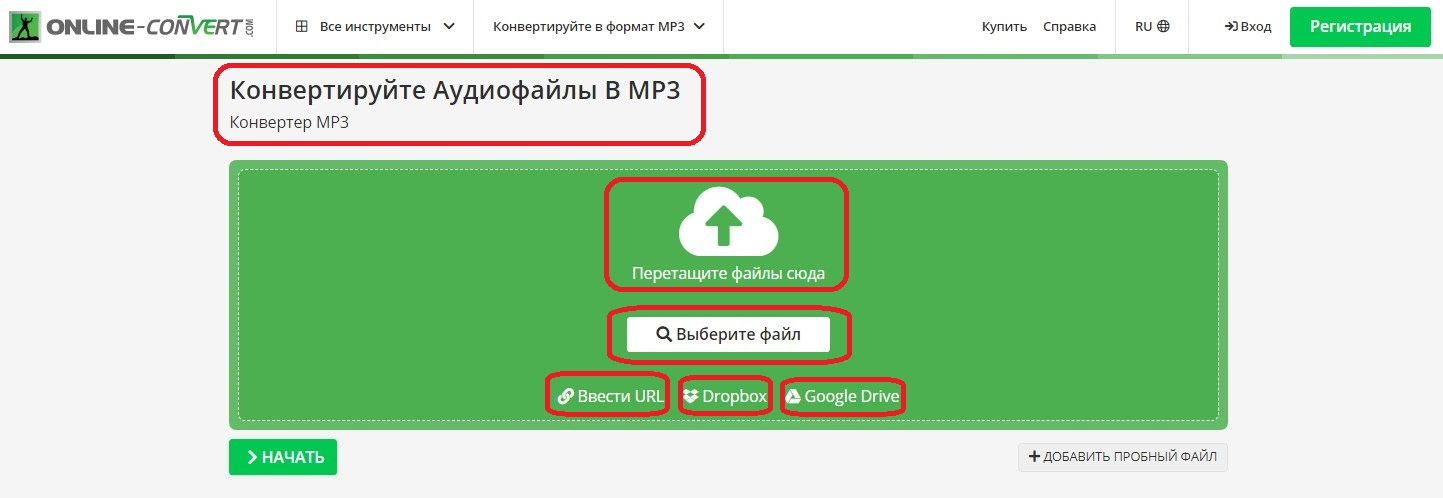
\includegraphics[width=0.8\textwidth]{img/cxp1.jpg}
\end{center}

В нашем примере мы видим, что есть 5 способов загрузить файл, который вам нужно конвертировать в mp3, на онлайн-сервис: найти в своем компьютере, взять с Dropbox, загрузить с Google-диска, загрузить с любого другого облачного хранилища или же просто перетащить в окошко загрузки, если папка с файлом уже открыта. Каждый сервис обозначен своим фирменным логотипом, а каждое действие – стандартным значком, обозначающим аналогичное действие на любом другом сайте.

По желанию пользователь может быстро ознакомиться с полным функционалом сайта, нажав меню «Все инструменты»:

\begin{center}
    
\includegraphics[width=0.8\textwidth]{img/cxp2.jpg}
\end{center}

В случае сомнений, нужен ли именно формат mp3 или какой-то другой, можно посмотреть все доступные форматы аудиофайлов:

\begin{center}
    
\includegraphics[width=0.8\textwidth]{img/cxp3.jpg}
\end{center}

Это пример соответствия ожиданиям пользователя, когда пользователь получает полный набор инструментов для своей дальнейшей работы и меньше чем за минуту знакомится с полным функционалом и возможностями сервиса.

\textbf{Видимость состояния системы}

Дизайн сайта, приложения, любого цифрового продукта должен быть построен так, чтобы пользователь всегда понимал, что сейчас происходит на сайте или в приложении, в какой части сайта или приложения он сейчас находится, насколько он приблизился к своей цели и каковы должны быть следующие действия.

Примером соблюдения принципа «видимости состояния системы» могут служить информационные уведомления наподобие «Выберите файл» и «Загрузка 50\%» на сайтах, где вы что-то загружаете или скачиваете. Это уведомления «Вы находитесь здесь» на сервисах с геолокацией, если вы разрешили доступ к данным о местоположении вашего гаджета. Такой интерфейс дает понимание, что делать дальше, и повышает доверие к цифровому продукту и бренду, предложившему этот продукт.

В рассмотренном выше примере, как только вы загрузили свой файл и нажали кнопку «Начать», появляется окошко с уведомлением, что «Ваш файл обрабатывается» и предупреждением «Не спешите. Страница результатов обновится автоматически»:

\begin{center}
    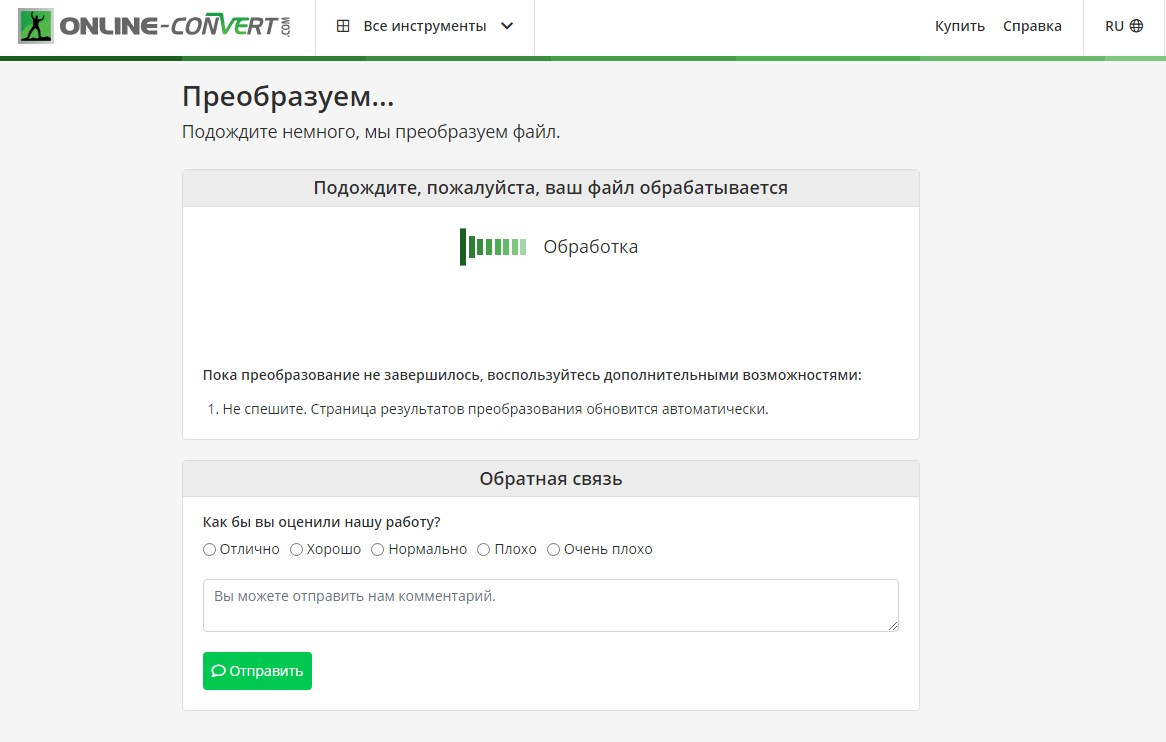
\includegraphics[width=0.8\textwidth]{img/cxp4.jpg}
\end{center}

Если вы уже обработали несколько файлов и вам скучно ждать, можно поставить оценку сервису или написать коротенький отзыв. Заметьте, сервис предоставляет такую возможность как бы «между делом», не забирая у пользователя его драгоценное время, когда он уже закончит работу с файлами, и не докучая потом сообщениями в духе «Оставьте отзыв».

\textbf{Пользовательский контроль и свобода}

Вероятность что-то не то нажать, не то загрузить или не то конвертировать есть всегда. У пользователя на каждом этапе должна быть возможность отменить действие либо удалить ошибочно загруженный или уже обработанный файл. В нашем примере сервис дает такую возможность с самого начала, как только пользователь загрузил свой файл на сайт, обозначив действие всем понятным значком в виде крестика и надписью «Удалить»:

\begin{center}
    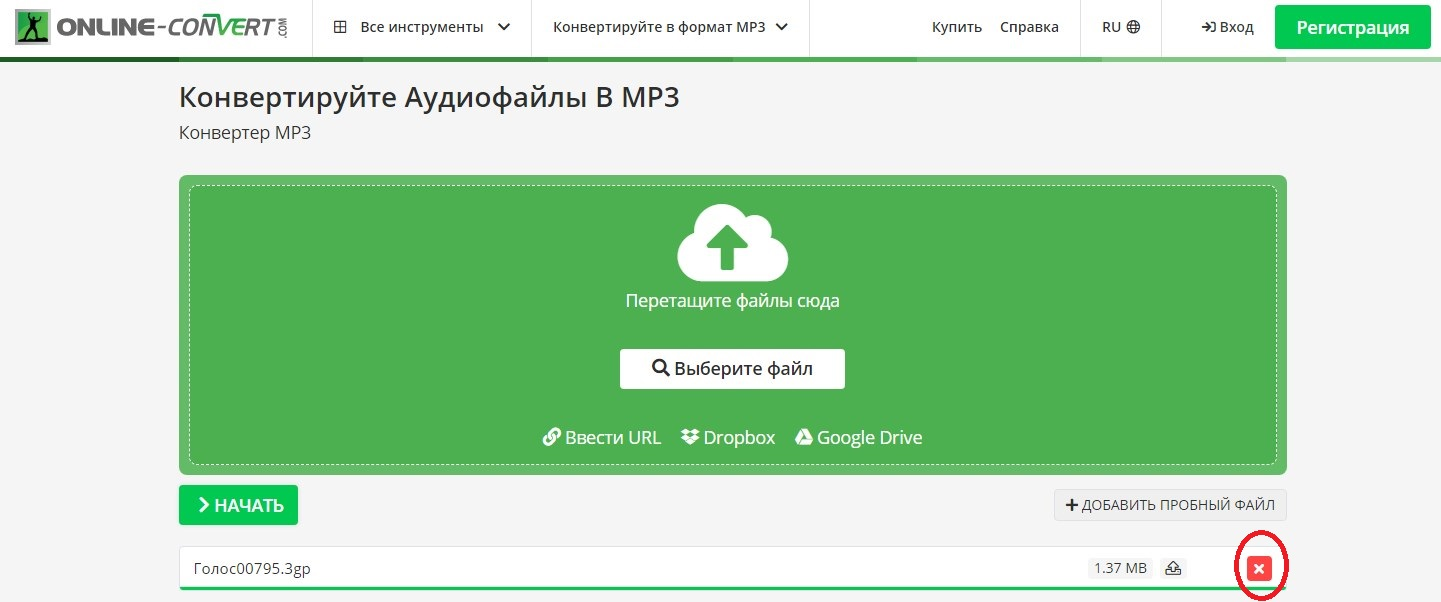
\includegraphics[width=0.8\textwidth]{img/cxp5.jpg}
\end{center}

Аналогичным образом можно поступить, если пользователь «спохватился» уже после того, как «отконвертил» файл. Помимо кнопок «Скачать» и «Загрузить в облако» есть кнопка «Удалить»:

\begin{center}
    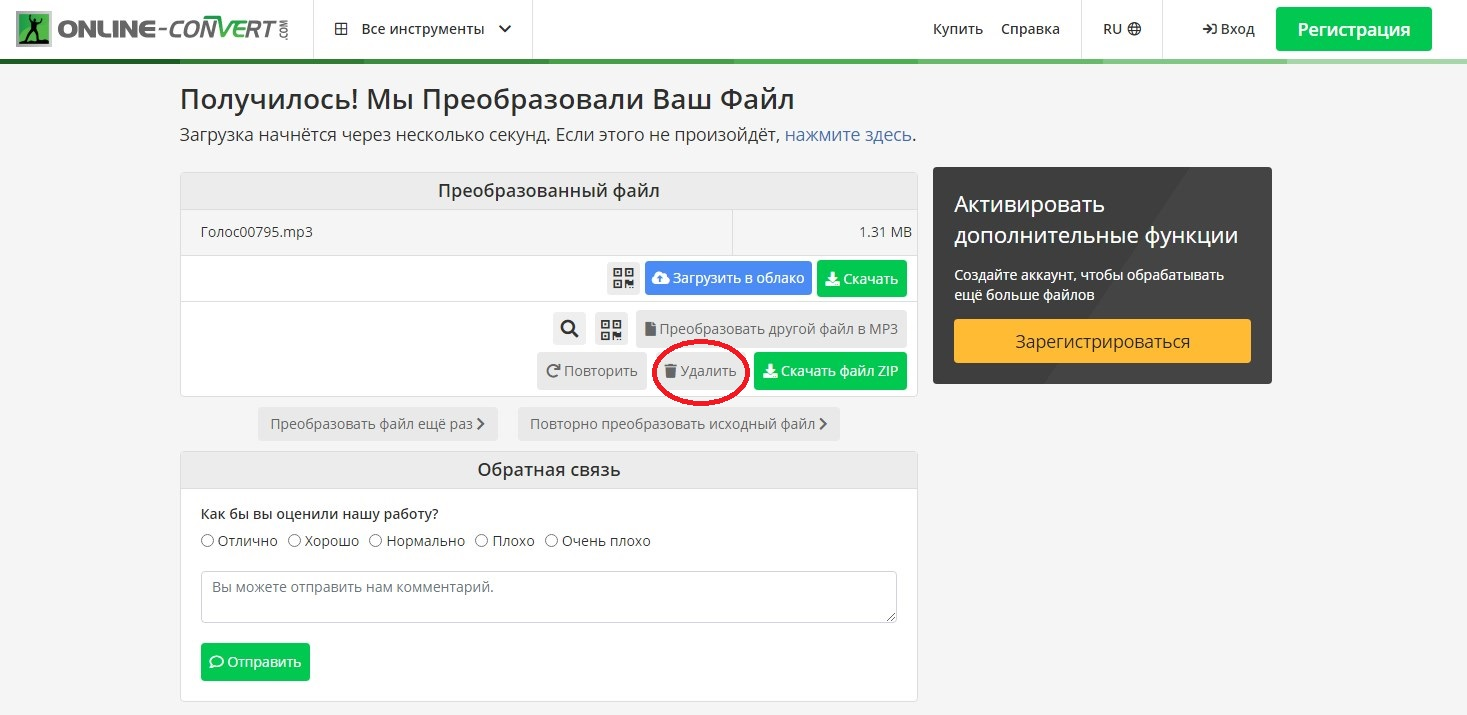
\includegraphics[width=0.8\textwidth]{img/cxp6.jpg}
\end{center}

Заметьте, что, если кнопки скачивания и загрузки выделены яркими броскими цветами, кнопка «Удалить» бледно-серая, дабы рука не тянулась к ней просто так, и пользователь не удалил готовый файл по ошибке.


\textbf{Предотвращение ошибок}

В продолжение темы следует сказать о предотвращении ошибок. Разумеется, никто не может застраховать пользователя от случайного нажатия кнопки и загрузки «не того» файла, однако обязанность разработчиков системы защитить пользователя от утечки данных и дать возможность в любой момент удалить данные не для широкого круга.

Если речь идет о более серьезных сервисах, связанных с денежными операциями, вариантом защиты может быть требование подтвердить ту или иную операцию (перевода денег, конвертации валюты и т.д.) Тут важно расставить приоритеты: сначала исключить серьезные ошибки, а затем минимизировать вероятность мелких неточностей.

Так, в нашем примере пользователь может не понять, что значить «Добавить пробный файл» и нажать эту кнопку из любопытства. Собственно, ничего страшного не происходит, и пользователь, убедившись, что это просто файл для демонстрации, как работает конвертер, может его сразу же удалить, не задерживаясь долго на странице и не отвлекаясь от своей основной задачи:

\begin{center}
    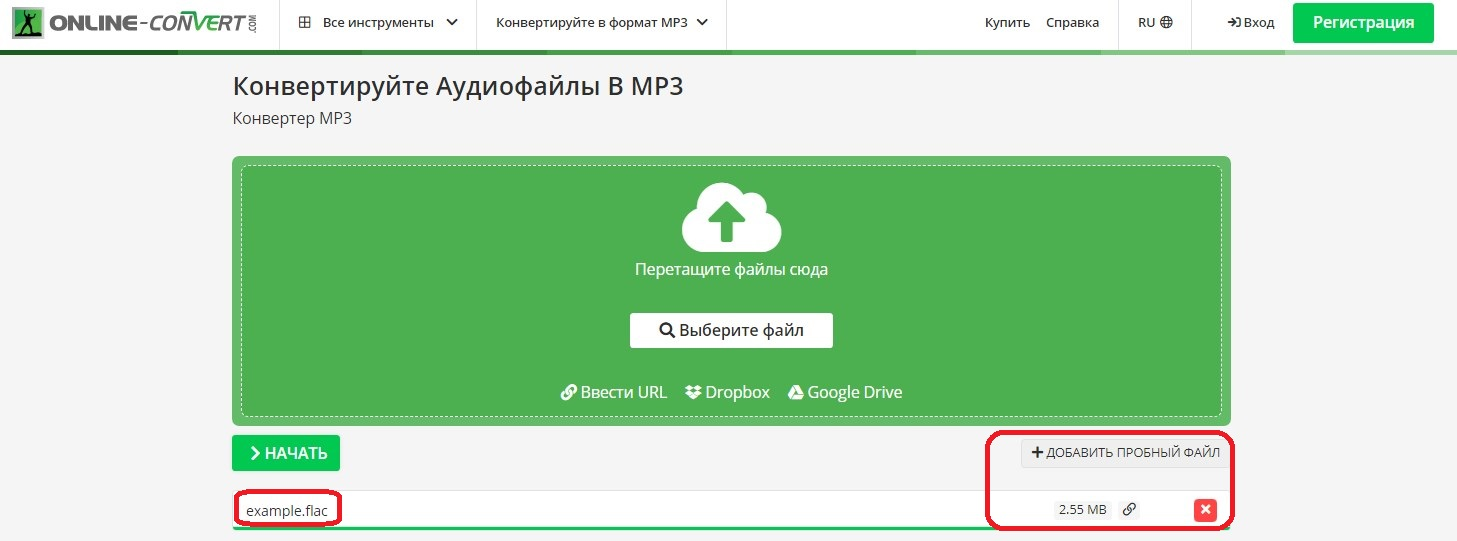
\includegraphics[width=0.8\textwidth]{img/cxp7.jpg}
\end{center}

Такие продуманные варианты предотвращения и исправления ошибок помогают «не выпадать» из стандартной последовательности действий.

\textbf{Последовательность и стандарты}

Любой продвинутый пользователь, вынужденно или добровольно проводящий онлайн по несколько часов в день, накапливает определенный опыт взаимодействия с цифровыми продуктами, а заодно и определенный массив ожиданий, как это взаимодействие должно происходить. Мы уже поговорили про соответствие ожиданиям пользователя с самого начала взаимодействия, но этого мало.

Соответствие стандартам и традиционной последовательности операций должна наблюдаться на всех этапах взаимодействия. Интерфейс может (и должен!) подсказывать возможные действия на шаг вперед, но ни в коем случае не опережать их и не сбивать с толку. В нашем случае вполне логично, что кнопка «Начать» появляется одновременно с кнопками загрузки файла. Так пользователю не нужно гадать, что будет дальше, когда он загрузит свой файл.

Аналогичным образом весь список возможных действий должен быть представлен по окончании каждого этапа. Например, после конвертации файла помимо кнопок «Скачать», «Загрузить» и «Удалить» появляется кнопка «Преобразовать следующий файл», чтобы пользователь не раздумывал, что ему делать дальше, если ему нужно конвертировать несколько файлов:


\begin{center}
    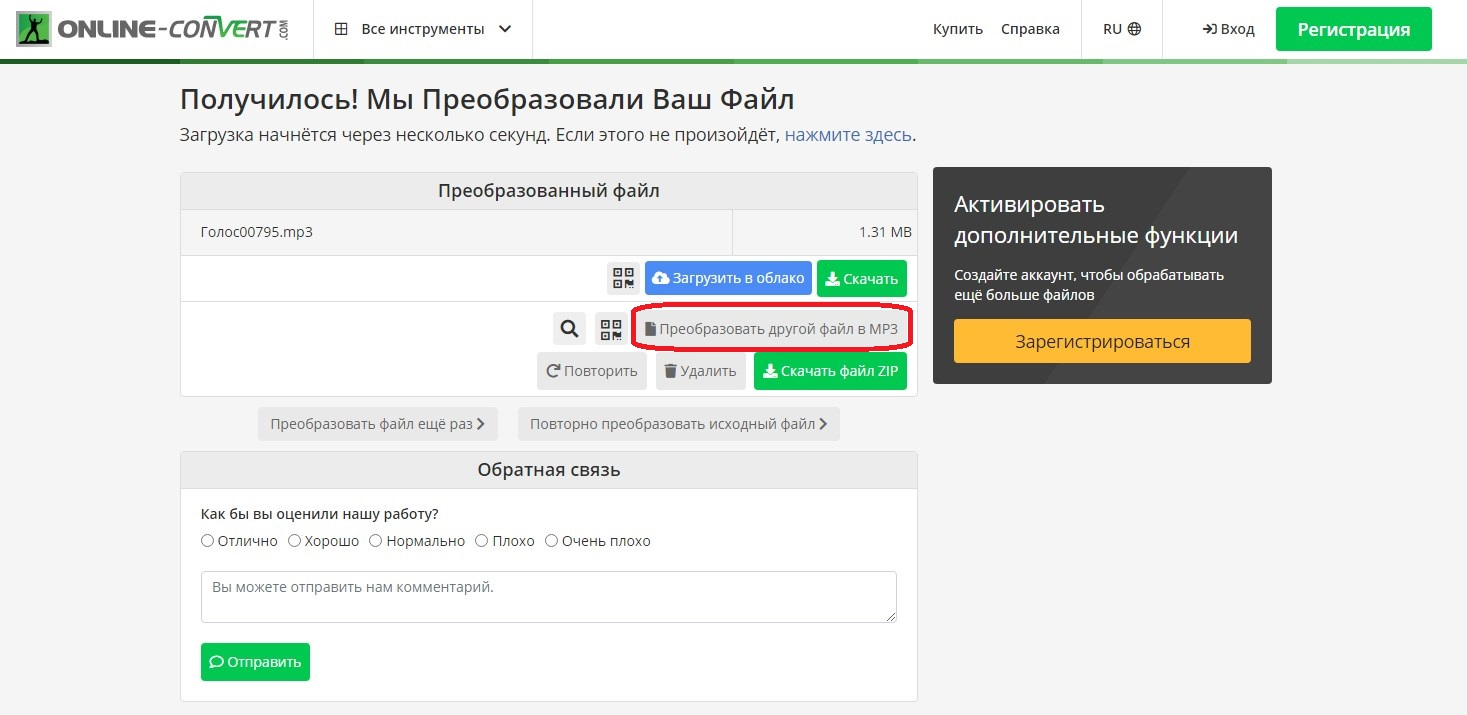
\includegraphics[width=0.8\textwidth]{img/cxp8.jpg}
\end{center}

Якоб Нильсен в своей статье отмечает, что неспособность сервиса поддерживать ожидаемую последовательность действий увеличивает когнитивную нагрузку на пользователей, когда это совершенно ни к чему [J. Nielsen, 2020]. Это примерно как стойка регистрации в отеле, что всегда расположена в холле. Если ее пришлось бы искать где-то через два коридора на другом этаже, это бы изрядно «напрягало» постояльцев отеля.

\textbf{Узнаваемость и напоминание}

Этот пункт «пересекается» с предыдущим. Чем более знакомым покажется пользователю интерфейс сайта, тем быстрее он на нем «освоится» и с тем большей вероятностью начнет заходить на этот сайт чаще. Особенно, если основной функционал сайта оправдает его ожидания.

Но данный пункт не только об этом. Он еще и том, чтобы снизить когнитивную нагрузку на пользователя даже в мелочах. Гипотетически юзер, конечно, должен помнить, какой именно файл он загрузил для конвертации минуту тому назад. Однако человека могут отвлечь какие-то дела, мысли, звонки. А если файлов много, можно просто сбиться со счета, потому как бесплатный сегмент сервиса позволяет конвертировать не более одного файла за один заход.

Именно поэтому основная информация об операции должна дублироваться на каждой странице каждого последующего шага. В нашем случае пользователь видит название загруженного файла как собственно при загрузке, так и после обработки:

\begin{center}
    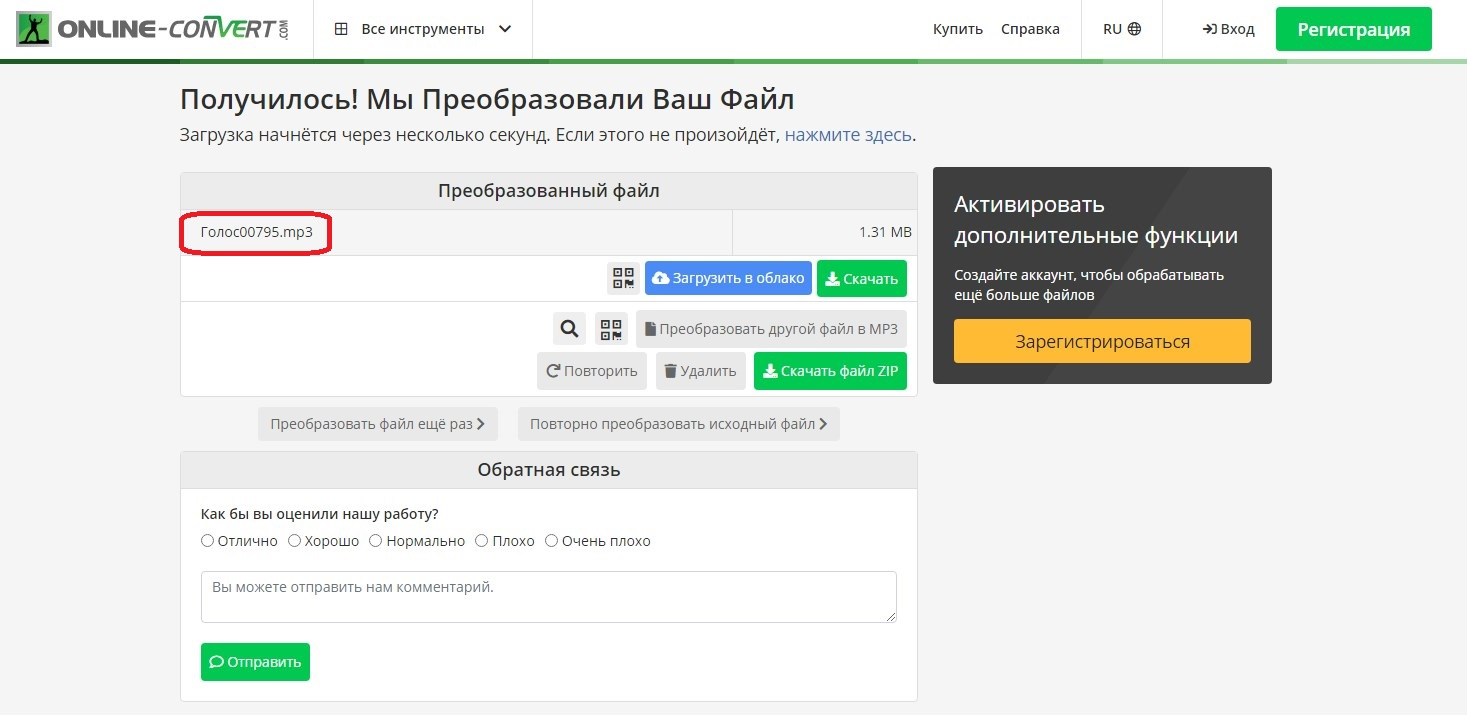
\includegraphics[width=0.8\textwidth]{img/cxp9.jpg}
\end{center}

К слову, это относится не только к оперативной информации, которая должна быть «на виду» и «под рукой». Аналогичным образом следует выстроить справочное сопровождение и помощь, предлагая ее в контексте возникшей проблемы, а не сразу весь мануал, 95\% из которого пользователю никогда не понадобится.


\textbf{Справочная информация}

Тем не менее, у пользователя должна быть возможность в любой момент найти ответ на любой свой вопрос, пусть даже пока у него никаких проблем не возникло. Раздел «Справка» должен быть на видном месте, лучше в верхнем меню, и структурирован на основные темы запросов пользователей:

\begin{center}
    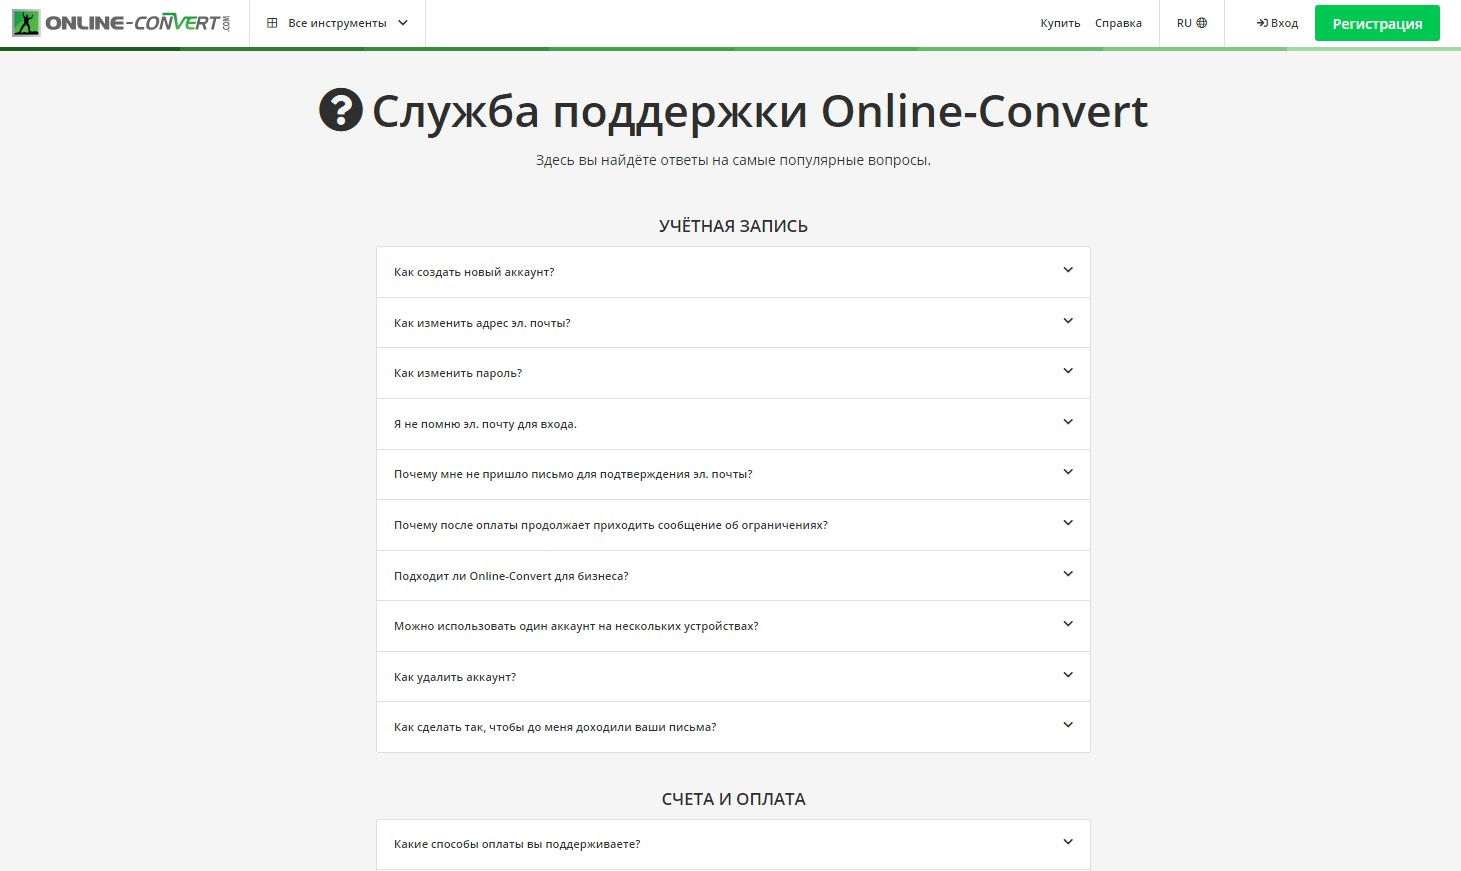
\includegraphics[width=0.8\textwidth]{img/cxp10.jpg}
\end{center}

Это, кстати, существенно разгрузит службу технической поддержки, потому что основной массив вопросов составляют одни и те же часто повторяющиеся проблемы, зачастую не имеющие никакого отношения собственно к сервису, а обусловленные человеческим фактором (забыл, не помню, не понял и т.д.). Разумеется, такого рода вопросы тоже должны быть обеспечены ответами.

\textbf{Гибкость использования}

Про индивидуальный подход слышали все, но не все разработчики вняли. Так, гибкость процессов – это «наше все». Не нужно «грузить» человека, которому нужно конвертировать один файл, информацией о годовой подписке. Эту информацию нужно предоставить только зарегистрированным пользователям.

Следует внятно написать, что именно даст регистрация на сайте и зачем она в принципе нужна. Например, для того, чтобы за один заход обрабатывать больше файлов, а не один, как в бесплатной версии:

\begin{center}
    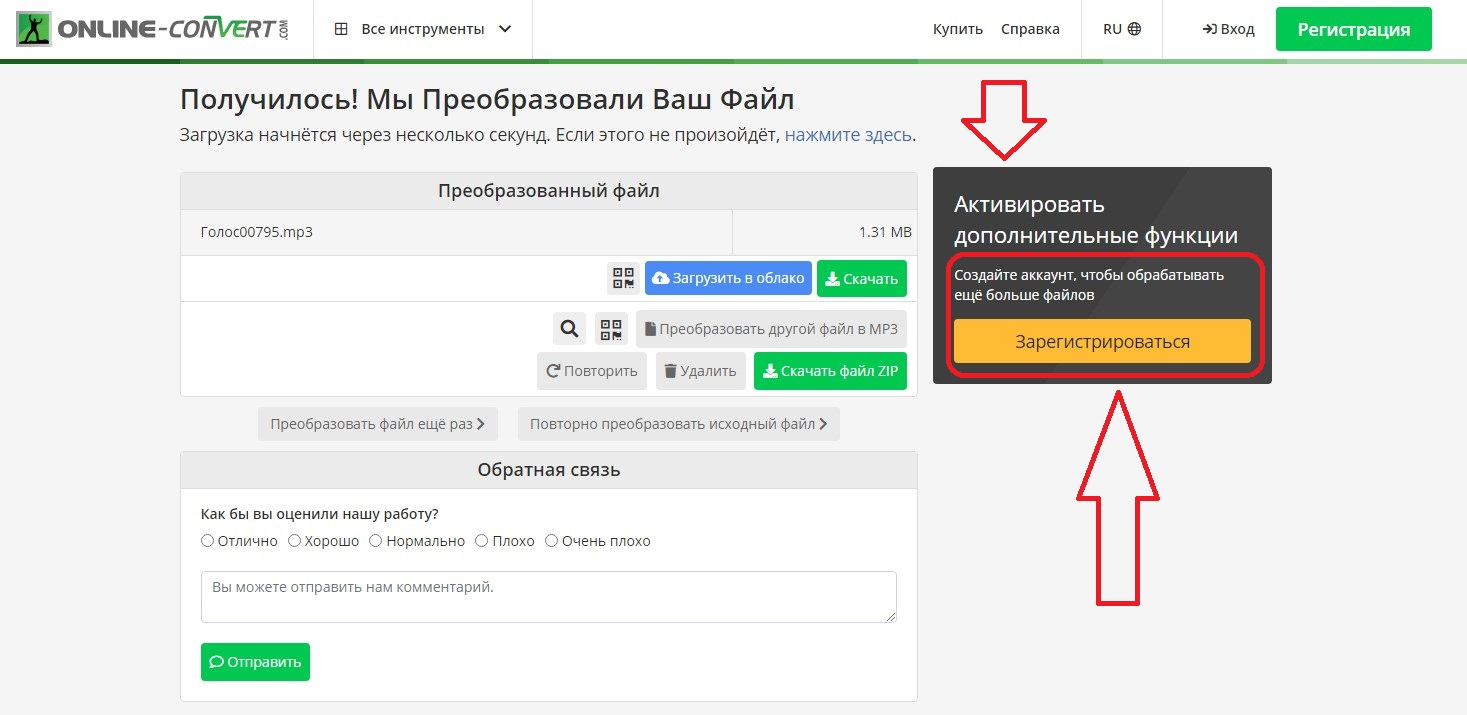
\includegraphics[width=0.8\textwidth]{img/cxp11.jpg}
\end{center}

Такая прозрачность избавит пользователя от возможных разочарований, а владельцев сайта – от негативных отзывов недовольных посетителей, потративших время на регистрацию непонятно зачем.

\textbf{Минимализм в дизайне}

Данный пункт связан со всеми предыдущими пунктами сразу. Если держать в фокусе только актуальную необходимую информацию, текущее действие и следующие возможные шаги, нет никакой необходимости перегружать сайт лишней информацией, картинками, элементами дизайна. Вот и не перегружайте.

Выражаясь научным языком, каждая дополнительная единица информации в интерфейсе конкурирует с другими единицами информации, в результате чего снижается относительная видимость каждой единицы информации [J. Nielsen, 2020].


\textbf{Помощь пользователям}

Про помощь пользователям в обращении с интерфейсом и использовании сервиса мы поговорили достаточно подробно. Однако могут возникнуть не зависящие от владельца сайта обстоятельства, мешающие воспользоваться сервисом. Например, прервется онлайн-соединение.

Сообщить об этом нужно простым и понятным языком: «Проверьте подключение к Интернету». Лучше не писать «Нет Интернета», потому что так пользователю может быть не совсем понятно, у кого именно нет интернет-соединения: у него или у вас.

Это и есть 10 эвристик юзабилити для дизайна пользовательского интерфейса. К слову, первоначальный вариант статьи Якоб Нильсен написал в далеком 1994 году, а в 2020 году только дополнил и расширил статью с учетом актуальной информации. Тем не менее, все базовые постулаты остались прежними. Как метко заметил автор, если что-то работает и остается неизменным на протяжении почти 30 лет, весьма вероятно, что это будет актуально еще достаточно долго.

Так что все эти рекомендации лучше соблюдать. В противном случае можно наделать много досадных ошибок, которые будут снижать конверсию и отпугивать пользователей.

\textbf{Основные ошибки в дизайне по Нильсену}

Какие ошибки можно совершить, проектируя дизайн интерфейса? Подробно об этом рассказал сам Якоб Нильсен в своей работе Top 10 Mistakes in Web Design («Топ-10 ошибок в веб-дизайне») [J. Nielsen, 2011]. Тут очень много самоочевидного, но почему-то все еще не воспринимаемого дизайнерами, разработчиками и заказчиками цифровых продуктов. Поэтому ограничимся просто списком с короткими пояснениями.

Топ-10 ошибок в веб-дизайне:

\begin{enumerate}
    \item Неудобный поиск – когда невозможно ничего найти, когда результат поиска нерелевантен запросу, когда на короткий внятный вопрос «выпадает» мануал на 150 страниц и т.д.
    \item PDF-файлы для онлайн-чтения – они оптимизированы под формат А4, а не под размер экрана, из-за чего возникает множество неудобств, начиная от мелкого шрифта и заканчивая неудобной прокруткой.
    \item Ранее просмотренные пользователем ссылки не меняют цвет – в итоге легко запутаться, особенно, если на сайте много контента.
    \item Нечитаемый текст – отсутствие разбивки на абзацы, слишком длинные абзацы, отсутствие разделов, подразделов и какой-то внятной структуры, избыток узкоспециальных терминов и профессионального жаргона.
    \item Фиксированный размер шрифта – не подходит для людей с не очень хорошим зрением, не желающим носить очки.
    \item Сходство с рекламой – если какой-либо раздел сайта похож на рекламу, его с высокой долей вероятности просто не станут изучать.
    \item Появление новых окон в браузере – это примерно как с рекламой, поэтому даже очень нужное окно чата с ботом лучше предлагать не сразу, а хотя бы через полминуты, чтобы пользователь успел «осмотреться» на сайте.
    \item Вопросы без ответов – когда ответ нельзя найти ни через поиск, ни через бот, ни через раздел «Справка», ни собственно в разделе сайта. Либо когда отсутствует информация, которая должна наличествовать по умолчанию. Например, цена товара в интернет-магазине.
    \item Нарушение общепринятых правил дизайна – меню должно быть вверху, строка поиска тоже вверху, кнопка «В корзину» вверху справа и т.д. Если такие общепонятные вещи приходится искать непонятно где, пользователь чаще всего просто уходит с сайта.
    \item Заголовки страниц не оптимизированы под поисковые системы – есть риск, что в этом случае даже очень ценная информация так и не попадет к пользователю. «Добро пожаловать» и «Внимание» не подходят, равно как и «Интересное предложение», «Акция», «Скидка» без пояснений, к чему это все относится.
\end{enumerate}

Небольшая подсказка к последнему пункту: заголовок страницы содержится внутри HTML-тега и почти всегда используется в качестве кликабельного заголовка среди результатов выдачи поисковых систем (SERP). Это для тех, кто хочет заняться оптимизацией сайта лично.

Итак, мы достаточно подробно рассмотрели все нюансы закона Якоба Нильсена. Осталось только им безоговорочно следовать… Или нет?.. Некоторые считают, что нет.


\textbf{Нюансы интерпретации закона Якоба Нильсена}

Сразу скажем, откуда взялся скептицизм в отношении закона Якоба Нильсена. И, кстати, не только в отношении него. Есть такая интересная статья «Ошибки в интерпретации UX законов: неверно понятые правила UX» [Р. Наджафов, 2022]. Тут, правда, больше не об ошибках, а о том, что все хорошо в меру.

Закон Якоба Нильсена частенько интерпретируют как призыв к примитивизму, отказу от эксперимента и креатива, использованию готовых шаблонов на все случаи жизни, потому что пользователям нужен узнаваемый дизайн, интуитивно понятный функционал и т.д. Имел ли это в виду сам Якоб Нильсен?

Вряд ли, потому что удобная навигация по сайту и креативные картинки к статьям в блоге никоим образом не исключают друг друга. Кроме того, вполне можно как-то нешаблонно сказать пользователю «Спасибо» за то, что он воспользовался вашим сервисом, когда он уже получит желаемый результат и точно не отвлечется от процесса на картинку с котиком, вручающим ему букет цветов.

Кроме того, новые впечатления поднимают настроение, а за хорошим настроением пользователь всегда охотно вернется на понравившийся сайт. Поэтому повторимся, что все хорошо в меру, во всем нужен баланс, а шаблоны и стандарты нужны исключительно для обеспечения удобства пользования.